\documentclass[14pt, a4paper]{extarticle}
\usepackage{mospolytech_coursework}

% ---------------------------------------------------------------------------
% Дополнительные пакеты, нужные для таблиц и диаграмм
% ---------------------------------------------------------------------------
\usepackage{ragged2e}        % для \RaggedRight в ячейках таблиц
\usepackage{tikz}
\usetikzlibrary{positioning, shapes.multipart, shapes.geometric,
                arrows.meta, fit, calc, backgrounds, shadows.blur}

% --- Брендовая палитра проекта pcshop (используется во всех диаграммах) ---
\definecolor{brandBlue}{HTML}{1F3B73}
\definecolor{brandBlueSoft}{HTML}{DBE5F5}
\definecolor{brandOrange}{HTML}{FF7A00}
\definecolor{brandOrangeSoft}{HTML}{FFE6CF}
\definecolor{brandGreen}{HTML}{2E8B57}
\definecolor{brandGreenSoft}{HTML}{D6EFE0}
\definecolor{brandRed}{HTML}{D9534F}
\definecolor{brandRedSoft}{HTML}{FBE0DF}
\definecolor{brandTeal}{HTML}{0EA5A5}
\definecolor{brandTealSoft}{HTML}{CFEFEF}
\definecolor{brandPurple}{HTML}{6D28D9}
\definecolor{brandPurpleSoft}{HTML}{E5DBF8}
\definecolor{brandLight}{HTML}{F4F6F8}
\definecolor{brandDark}{HTML}{1F2937}

% ---------------------------------------------------------------------------
% Определение данных
% ---------------------------------------------------------------------------
\newcommand{\theme}{%
    Разработка веб-приложения для учёта комплектующих,
    сборки и продажи персональных компьютеров%
}
\newcommand{\subject}{Разработка веб-приложений}
\newcommand{\student}{Ануфриев Платон Дмитриевич}
\newcommand{\group}{241-327}
\newcommand{\teacher}{Кружалов Алексей Сергеевич}

\begin{document}

% ── Титульный лист ──────────────────────────────────────────────────────────
\thispagestyle{empty}

\begin{center}
    {\small МИНИСТЕРСТВО НАУКИ И ВЫСШЕГО ОБРАЗОВАНИЯ РОССИЙСКОЙ ФЕДЕРАЦИИ}
    
    \resizebox{\textwidth}{!}{\fontsize{8pt}{10pt}\selectfont ФЕДЕРАЛЬНОЕ 
    ГОСУДАРСТВЕННОЕ АВТОНОМНОЕ ОБРАЗОВАТЕЛЬНОЕ УЧРЕЖДЕНИЕ ВЫСШЕГО ОБРАЗОВАНИЯ} 
    
    {\small \textbf{«МОСКОВСКИЙ ПОЛИТЕХНИЧЕСКИЙ УНИВЕРСИТЕТ»}} \\
    {\small \textbf{(МОСКОВСКИЙ ПОЛИТЕХ)}}

    \vspace{4cm}

    {\Large \textbf{КУРСОВОЙ ПРОЕКТ}} \\[1cm]
    {\large по курсу \\ «\subject»}

    \vspace{1.5cm}

    \textbf{ТЕМА} \\[0.3cm]
    {\large «\theme»}

    \vspace{3cm}

    % Блок подписей (сдвинут вправо)
    \hfill
    \begin{tabular}{p{3cm} l}
        \textbf{Выполнил:} & \student \\
        \textbf{Группа:}   & \group \\
        \\
        \textbf{Проверил:}  & \teacher
    \end{tabular}

    \vfill

    Москва, 2026

\end{center}
\newpage

% ── Задание ──────────────────────────────────────────────────────────────────
\IfFileExists{task.pdf}{\includepdf[pages=-]{task.pdf}}{}

% ── Содержание ───────────────────────────────────────────────────────────────
\tableofcontents

% ── Введение ─────────────────────────────────────────────────────────────────
\phantomsection
\section*{Введение}
\addcontentsline{toc}{section}{Введение}

\textbf{Актуальность темы.} Рынок персональных компьютеров активно развивается, а спрос на индивидуальные сборки ПК стабильно сохраняется: пользователи заинтересованы в получении устройств, максимально соответствующих их требованиям по производительности, стоимости, внешнему виду и назначению. Это приводит к росту числа небольших компаний и частных специалистов, занимающихся продажей комплектующих, сборкой компьютеров под заказ и сервисным сопровождением. Для таких организаций критически важна автоматизация процессов учёта комплектующих, формирования сборок, оформления заказов и анализа результатов продаж: при отсутствии специализированной информационной системы возникают проблемы с контролем остатков на складе, отслеживанием движения товаров, ведением клиентских заказов и расчётом прибыли.

\textbf{Степень разработанности проблемы.} На рынке представлено множество интернет-магазинов компьютерной техники (DNS, «Регард», «НИКС», «Ситилинк») и универсальных CRM-/ERP-систем. Однако существующие решения либо ориентированы на крупный розничный сегмент и не учитывают специфику внутреннего учёта комплектующих при сборке ПК под заказ, либо избыточны и дороги для малого бизнеса. Это обуславливает целесообразность разработки специализированного веб-приложения, объединяющего функции каталога, склада, конфигуратора, заказов и аналитики в едином интерфейсе с разграничением прав доступа.

\textbf{Объект исследования} --- процессы учёта комплектующих, сборки и продажи персональных компьютеров в малых компаниях.

\textbf{Предмет исследования} --- веб-приложение, предназначенное для автоматизации учёта комплектующих, управления сборками ПК и оформления заказов с разграничением прав доступа по ролям.

\textbf{Целью данной работы} является проектирование и реализация веб-приложения, обеспечивающего автоматизацию учёта комплектующих, управление сборками ПК и взаимодействие администраторов, менеджеров и клиентов через систему личных кабинетов.

\textbf{Для достижения цели} необходимо решить следующие задачи:
\begin{itemize}
    \item провести анализ предметной области и обзор существующих программных решений;
    \item обосновать выбор технологического стека для разработки;
    \item спроектировать архитектуру приложения, модель данных и пользовательские интерфейсы;
    \item реализовать аутентификацию, ролевую модель и CRUD-операции над основными сущностями;
    \item реализовать конфигуратор сборки, аналитические отчёты, импорт и экспорт данных;
    \item выполнить развёртывание приложения и оформить пояснительную записку.
\end{itemize}

\textbf{Практическая значимость} работы заключается в создании готового к внедрению программного продукта, который может использоваться действующими магазинами комплектующих и небольшими сборщиками ПК для автоматизации ключевых бизнес-процессов и сокращения операционных издержек.

% ── Глава 1 ──────────────────────────────────────────────────────────────────
\phantomsection
\section*{Глава 1. Анализ предметной области}
\addcontentsline{toc}{section}{Глава 1. Анализ предметной области}
\stepcounter{section}

\subsection{Анализ предметной области сборки и продажи ПК}

Предметная область курсового проекта связана с деятельностью по закупке, хранению, учёту, сборке и продаже персональных компьютеров. Такая деятельность объединяет несколько взаимосвязанных процессов: работу со складом комплектующих, подбор совместимых компонентов, формирование готовых конфигураций, оформление заказов, взаимодействие с клиентами и получение аналитической информации по продажам.

Основой процесса является \textbf{складской учёт}. На складе могут находиться процессоры, материнские платы, видеокарты, оперативная память, накопители, блоки питания, корпуса, системы охлаждения и иные комплектующие. Для каждого товара необходимо хранить его наименование, категорию, количество, закупочную стоимость, продажную цену, характеристики и текущий статус наличия. При отсутствии автоматизированной системы ведение такого учёта вручную приводит к ошибкам, дублированию данных и трудностям при обновлении информации.

Следующий важный процесс --- \textbf{сборка персонального компьютера}. В отличие от обычной продажи единичных товаров, сборка ПК требует учёта совместимости комплектующих, контроля остатков и фиксации состава каждой конфигурации. При формировании одной сборки используются сразу несколько единиц товаров из разных категорий. После подтверждения сборки количество соответствующих комплектующих на складе должно автоматически уменьшаться, что требует поддержки связи между складским учётом и сущностью сборки.

Ещё одним ключевым направлением является \textbf{работа с заказами}. Клиент может выбрать готовую конфигурацию, заказать сборку по своим параметрам либо приобрести отдельные комплектующие. Для каждого заказа требуется сохранять сведения о клиенте, составе заказа, дате оформления, сумме, статусе исполнения и способе оплаты. Кроме того, важно обеспечить возможность отслеживания истории заказов и формирования отчётных данных по продажам.

В рамках данной предметной области можно выделить несколько \textbf{категорий пользователей}. Администратор отвечает за полное управление системой, настройку справочников и управление доступом. Менеджер работает с товарами, заказами и клиентами, а также может создавать и редактировать сборки. Клиент взаимодействует с приложением как пользователь, который просматривает ассортимент, выбирает товары и оформляет заказ. Следовательно, в системе должна быть реализована ролевая модель доступа.

Особенностью данной предметной области является необходимость обработки \textbf{аналитической информации}: пользователю системы важно не только добавлять и изменять записи, но и получать агрегированные данные --- общую сумму продаж за период, количество проданных товаров, наиболее востребованные комплектующие, остатки на складе, прибыль по заказам и по готовым сборкам.

Таким образом, предметная область включает совокупность процессов учёта товаров, формирования сборок, сопровождения заказов и анализа результатов продаж. Это делает разработку специализированного веб-приложения целесообразной и практически значимой.

\subsection{Обзор существующих веб-приложений и интернет-магазинов}

На современном рынке существует большое количество интернет-магазинов компьютерной техники и платформ для продажи комплектующих. К числу наиболее известных относятся крупные магазины, предлагающие широкий каталог товаров, фильтрацию по характеристикам, оформление заказов и базовые элементы личного кабинета пользователя. Такие решения ориентированы прежде всего на массовую торговлю и онлайн-продажи.

Несмотря на широкую распространённость подобных систем, они не всегда подходят для задач малого бизнеса или индивидуальной сборки ПК под заказ. Во многих случаях веб-сервисы ориентированы только на витрину товаров и не предоставляют полноценного механизма внутреннего учёта комплектующих, отслеживания фактических остатков или ведения истории использования компонентов в конкретных сборках.

Отдельно следует отметить \textbf{конфигураторы ПК}, позволяющие подобрать комплектующие по категориям. Их преимущество заключается в помощи пользователю при формировании конфигурации, однако подобные системы часто не интегрированы с внутренним складским учётом и механизмом управления заказами. В результате владелец бизнеса вынужден использовать сразу несколько разрозненных инструментов: отдельно таблицы для склада, отдельно мессенджеры или CRM для клиентов и отдельно сайт для публикации товаров.

Также существуют \textbf{универсальные CRM- и ERP-системы}, которые могут использоваться для учёта товаров и заказов. Их достоинством является наличие модулей для управления клиентами и продажами. Однако такие решения часто являются избыточными по функциональности, сложны в настройке и адаптации под конкретный сценарий сборки персональных компьютеров, а их использование может быть экономически невыгодным для небольших проектов.

Для наглядного сопоставления существующих программных продуктов проведён сравнительный анализ четырёх характерных представителей рынка: крупного интернет-магазина электроники DNS, специализированной сети «Регард», магазина-конфигуратора «НИКС» и универсальной торговой площадки «Ситилинк». Сравнение по существенным для предметной области критериям приведено в таблице~\ref{tab:competitors}.

\begin{table}[ht!]
\caption{Сравнительный анализ существующих веб-приложений}
\label{tab:competitors}
\footnotesize
\begin{tabularx}{\textwidth}{|>{\RaggedRight\arraybackslash}p{0.30\textwidth}|>{\centering\arraybackslash}X|>{\centering\arraybackslash}X|>{\centering\arraybackslash}X|>{\centering\arraybackslash}X|>{\centering\arraybackslash}X|}
\hline
\textbf{Критерий} & \textbf{DNS} & \textbf{Регард} & \textbf{НИКС} & \textbf{Сити-линк} & \textbf{Разра-баты-ваемое} \\ \hline
Каталог комплектующих & + & + & + & + & + \\ \hline
Конфигуратор сборки ПК & + & --- & + & --- & + \\ \hline
Контроль совместимости комплектующих & частично & --- & + & --- & + \\ \hline
Внутренний учёт остатков на складе & --- & --- & --- & --- & + \\ \hline
Ведение заказов в едином интерфейсе & + & + & + & + & + \\ \hline
Ролевая модель (админ/менеджер/клиент) & --- & --- & --- & --- & + \\ \hline
Аналитика по продажам и прибыли & --- & --- & --- & --- & + \\ \hline
Импорт/экспорт каталога (CSV, Excel) & --- & --- & --- & --- & + \\ \hline
Адаптация под малый бизнес & низкая & низкая & сред-няя & низкая & полная \\ \hline
Стоимость использования для бизнеса & нет & нет & нет & нет & собств. \\ \hline
\end{tabularx}
\end{table}

Результаты сравнения подтверждают сделанный ранее вывод: ни одно из рассмотренных решений не покрывает в комплексе задачи внутреннего учёта комплектующих, конфигурирования сборок, ведения заказов и аналитики. Существующие веб-приложения ориентированы прежде всего на витрину товаров для конечного покупателя и не предоставляют инструментов работы для администратора и менеджера небольшой компании по сборке ПК. Это окончательно обосновывает целесообразность разработки собственного специализированного веб-приложения.

\subsection{Анализ программных инструментов разработки}

Для реализации веб-приложения необходимо выбрать стек технологий, который обеспечит сбалансированное соотношение скорости разработки, надёжности эксплуатации и удобства последующего сопровождения. В таблице~\ref{tab:tech} приведено сравнение основных программных инструментов, рассматривавшихся в качестве кандидатов для серверной части, клиентской части и хранилища данных.

\begin{table}[ht!]
\caption{Сравнение программных инструментов разработки}
\label{tab:tech}
\small
\begin{tabularx}{\textwidth}{|>{\RaggedRight\arraybackslash}p{0.18\textwidth}|>{\RaggedRight\arraybackslash}p{0.20\textwidth}|>{\RaggedRight\arraybackslash}X|>{\RaggedRight\arraybackslash}X|}
\hline
\textbf{Инструмент} & \textbf{Назначение} & \textbf{Преимущества} & \textbf{Недостатки} \\ \hline
Django (Python) & Серверный фреймворк & Встроенная админ-панель, ORM, миграции, аутентификация, формы и валидация & Меньшая гибкость по сравнению с микрофреймворками \\ \hline
Flask (Python) & Серверный микрофреймворк & Минимализм, гибкость, простой запуск & Отсутствие готовой админки, много ручной работы \\ \hline
Node.js + Express & Серверная платформа & Высокая производительность, единый язык с фронтендом & Отсутствие готовой ORM, ручная сборка инфраструктуры \\ \hline
Laravel (PHP) & Серверный фреймворк & Зрелая экосистема, богатый набор пакетов & Менее распространён в российских учебных проектах \\ \hline
Bootstrap 5 & CSS-фреймворк & Готовая адаптивная сетка, набор компонентов, быстрый старт & Типовой вид интерфейса без кастомизации \\ \hline
Vanilla JS & Клиентская логика & Отсутствие зависимостей, простота отладки & Ручная реализация повторяющихся компонентов \\ \hline
React / Vue.js & Клиентские фреймворки & Компонентный подход, удобство для SPA & Усложняют сборку и SEO в учебном проекте \\ \hline
PostgreSQL & СУБД & Сложные запросы, надёжная транзакционная модель, ограничения целостности & Требует более тщательной настройки \\ \hline
SQLite & СУБД & Не требует сервера, удобна для разработки & Ограниченная пропускная способность \\ \hline
Docker & Контейнеризация & Унификация окружения, простота деплоя & Дополнительный слой инфраструктуры \\ \hline
Git + GitHub & Контроль версий & История изменений, ревью кода, распределённая работа & Требует дисциплины ведения коммитов \\ \hline
\end{tabularx}
\end{table}

На основании проведённого сравнения для реализации курсового проекта выбран следующий технологический стек:
\begin{itemize}
    \item \textbf{серверная часть} --- язык программирования Python~3.12 и фреймворк Django~5. Выбор обусловлен наличием встроенной административной панели, ORM для описания модели данных, готовых механизмов аутентификации, авторизации и валидации форм, а также большим объёмом учебной и справочной литературы~\cite{hawkins2022django};
    \item \textbf{клиентская часть} --- HTML5, CSS3, CSS-фреймворк Bootstrap~5 и Vanilla JavaScript. Такой набор позволяет получить адаптивный интерфейс, не усложняя структуру проекта дополнительными сборщиками и SPA-фреймворками;
    \item \textbf{хранилище данных} --- реляционная СУБД PostgreSQL~16 в качестве основной СУБД и SQLite на этапе локальной разработки. PostgreSQL обеспечивает поддержку ограничений целостности, транзакций и сложных аналитических запросов;
    \item \textbf{вспомогательные библиотеки} --- Django REST framework для построения внутреннего API, библиотека openpyxl и стандартный модуль \texttt{csv} для импорта и экспорта данных, библиотека Pillow для работы с изображениями товаров;
    \item \textbf{инфраструктура и инструменты разработки} --- система контроля версий Git и хостинг репозитория GitHub, среда разработки PyCharm Community / VS~Code, контейнеризация средствами Docker и Docker Compose, обратный прокси-сервер Nginx и WSGI-сервер Gunicorn для последующего развёртывания приложения.
\end{itemize}

Выбранный стек удовлетворяет требованиям учебного проекта по дисциплине «Разработка веб-приложений», обеспечивает быстрый старт разработки за счёт готовых компонентов Django и Bootstrap и позволяет в дальнейшем масштабировать приложение без полной переработки исходного кода.

\subsection{Формулировка цели, задач и требований к системе}

На основе проведённого анализа предметной области, обзора существующих решений и анализа программных инструментов сформулированы требования к разрабатываемому веб-приложению.

\textbf{Цель работы} --- разработка веб-приложения для учёта комплектующих, сборки и продажи персональных компьютеров с разграничением прав доступа администраторов, менеджеров и клиентов.

В системе должны быть реализованы функции \textbf{регистрации, аутентификации и авторизации} пользователей. Это необходимо для разграничения доступа к возможностям приложения в зависимости от роли пользователя. Администратор должен иметь полный доступ ко всем разделам системы, менеджер --- доступ к управлению товарами, заказами и сборками, клиент --- доступ к просмотру каталога, оформлению заказов и просмотру своих данных.

Важным требованием является наличие \textbf{CRUD-интерфейса} для основных сущностей приложения. Пользователь с соответствующими правами должен иметь возможность создавать, просматривать, изменять и удалять записи о товарах, сборках, заказах и пользователях.

Разрабатываемое приложение должно содержать \textbf{не менее трёх основных сущностей}. В рамках данного проекта такими сущностями являются:
\begin{itemize}
    \item пользователи (с ролями);
    \item категории и комплектующие;
    \item сборки ПК и их состав;
    \item заказы и позиции заказов.
\end{itemize}

Кроме хранения и редактирования данных, система должна обеспечивать \textbf{обработку и агрегирование} информации: вычисление суммы продаж за период, определение количества товаров на складе, расчёт прибыли по заказам и отображение наиболее востребованных комплектующих.

Отдельным требованием является \textbf{поддержка загрузки и выгрузки файлов} в форматах CSV и Excel для импорта начального каталога, экспорта отчётных данных и резервного копирования.

К \textbf{нефункциональным требованиям} относятся удобство пользовательского интерфейса, надёжность хранения данных, безопасность (хранение паролей в виде хэшей, защита от CSRF, XSS, SQL-инъекций), расширяемость и достаточная производительность при работе с каталогом, заказами и сборками.

Таким образом, разрабатываемая система должна представлять собой веб-приложение, объединяющее в себе механизмы учёта товаров, формирования сборок ПК, оформления заказов, разграничения доступа, загрузки и выгрузки файлов, а также аналитической обработки данных.

% ── Глава 2 ──────────────────────────────────────────────────────────────────
\phantomsection
\section*{Глава 2. Проектирование веб-приложения}
\addcontentsline{toc}{section}{Глава 2. Проектирование веб-приложения}
\stepcounter{section}

Во второй главе курсовой работы выполняется проектирование разрабатываемого веб-приложения. На основании сформулированных в первой главе требований проводится анализ целевой аудитории и пользовательских ролей, формализуются функциональные и нефункциональные требования, описываются варианты использования и сценарии работы пользователей, проектируется модель данных приложения и разрабатываются макеты основных страниц.

\subsection{Анализ целевой аудитории и ролей пользователей}

Разрабатываемое веб-приложение ориентировано на небольшие компании и индивидуальных специалистов, занимающихся продажей комплектующих, сборкой персональных компьютеров под заказ и сопровождением заказов клиентов. Целевая аудитория системы делится на две принципиально разные группы: внутренние пользователи (сотрудники компании --- администратор и менеджер) и внешние пользователи (клиенты --- посетители сайта и зарегистрированные покупатели). Анализ предметной области показал, что в работе таких организаций задействованы три основные роли пользователей.

\textbf{Администратор.} Сотрудник, отвечающий за общее техническое сопровождение приложения, ведение справочников, управление учётными записями других пользователей и настройку параметров системы. Возрастной диапазон --- 22--40 лет, уверенный пользователь компьютера, ежедневно работает с системой с настольного устройства. Ключевые ожидания: быстрый доступ к административной панели, возможность массового изменения справочников, чёткое разграничение прав менеджеров и клиентов.

\textbf{Менеджер.} Основной операционный пользователь системы. В обязанности менеджера входит ведение каталога комплектующих, оформление и сопровождение заказов клиентов, формирование сборок ПК, контроль остатков на складе и подготовка отчётности. Возрастной диапазон --- 22--45 лет, средний и выше среднего уровень владения IT, работает с системой 6--8 часов в день преимущественно с настольного устройства. Ключевые ожидания: удобный CRUD-интерфейс для товаров, заказов и сборок; быстрый поиск по каталогу; наглядное отображение остатков; возможность импорта и экспорта данных.

\textbf{Клиент.} Конечный пользователь, для которого приложение является витриной товаров и средством оформления заказа. Возрастной диапазон --- 18--45 лет, уровень владения IT --- выше среднего. Использует приложение преимущественно с настольного устройства или планшета, частично --- с мобильного телефона. Ключевые ожидания: удобный фильтр и поиск товаров по характеристикам, возможность собрать конфигурацию ПК из совместимых комплектующих, оформление заказа без длительной регистрации, просмотр истории заказов в личном кабинете.

Отдельной категорией являются \textbf{гости} --- неавторизованные посетители сайта, имеющие доступ к публичному каталогу товаров и формам регистрации. Сводные характеристики ролей приведены в таблице~\ref{tab:roles}.

\begin{table}[ht!]
\caption{Сравнительные характеристики ролей пользователей}
\label{tab:roles}
\small
\begin{tabularx}{\textwidth}{|>{\RaggedRight\arraybackslash}p{0.16\textwidth}|>{\RaggedRight\arraybackslash}X|>{\RaggedRight\arraybackslash}p{0.20\textwidth}|>{\RaggedRight\arraybackslash}p{0.18\textwidth}|}
\hline
\textbf{Роль} & \textbf{Основные задачи} & \textbf{Частота использования} & \textbf{Устройство} \\ \hline
Администратор & Управление пользователями и ролями, настройка справочников, аналитика & Несколько раз в неделю, 1--2~ч в день & Настольный ПК \\ \hline
Менеджер & Ведение каталога, оформление заказов, формирование сборок, контроль остатков & Ежедневно, 6--8~ч в день & Настольный ПК / ноутбук \\ \hline
Клиент & Просмотр каталога, конфигурирование сборки, оформление заказа & 1--3 сессии при покупке & ПК, планшет, смартфон \\ \hline
Гость & Просмотр каталога, регистрация & Эпизодически & ПК, планшет, смартфон \\ \hline
\end{tabularx}
\end{table}

На основе перечня ролей построена матрица прав доступа к основным сущностям системы (таблица~\ref{tab:rbac}). Матрица фиксирует разрешённые операции: C --- создание, R --- чтение, U --- изменение, D --- удаление.

\begin{table}[ht!]
\caption{Матрица прав доступа (CRUD)}
\label{tab:rbac}
\small
\begin{tabularx}{\textwidth}{|>{\RaggedRight\arraybackslash}p{0.32\textwidth}|>{\centering\arraybackslash}X|>{\centering\arraybackslash}X|>{\centering\arraybackslash}X|>{\centering\arraybackslash}X|}
\hline
\textbf{Сущность / действие} & \textbf{Гость} & \textbf{Клиент} & \textbf{Мене\-джер} & \textbf{Адми\-нистра\-тор} \\ \hline
Каталог комплектующих & R & R & CRUD & CRUD \\ \hline
Готовые сборки ПК & R & R & CRUD & CRUD \\ \hline
Свой заказ & --- & CRU & RU & RUD \\ \hline
Чужие заказы & --- & --- & RU & RUD \\ \hline
Свой профиль (клиент) & --- & RU & R & RU \\ \hline
Учётные записи пользователей & --- & --- & --- & CRUD \\ \hline
Справочники (категории, статусы) & --- & --- & R & CRUD \\ \hline
Аналитические отчёты & --- & --- & R & R \\ \hline
\end{tabularx}
\end{table}

Полученные сведения о целевой аудитории и матрице прав доступа учитываются при проектировании пользовательских интерфейсов: для администратора и менеджера предусматривается интерфейс с большим количеством таблиц, фильтров и действий, ориентированный на работу с настольного устройства; для клиента --- более простой и адаптивный интерфейс с поддержкой мобильных устройств.

\subsection{Описание функциональности приложения}

На основе анализа предметной области, требований к системе и описанных пользовательских ролей сформирован перечень функциональных возможностей разрабатываемого веб-приложения. Функциональность представлена через перечень функциональных и нефункциональных требований, диаграмму вариантов использования, пользовательские истории и описание ключевых сценариев работы.

Действующими лицами (актёрами) системы являются: \emph{гость} --- неавторизованный посетитель сайта, \emph{клиент} --- зарегистрированный покупатель, \emph{менеджер} --- сотрудник, ведущий товары и заказы, \emph{администратор} --- сотрудник, имеющий полный доступ к системе.

Диаграмма вариантов использования (рисунок~\ref{fig:usecase}) объединяет в единой системе четыре актёра и пятнадцать прецедентов. Между ролями определены отношения наследования (клиент наследует возможности гостя, администратор --- возможности менеджера), а между прецедентами «Оформление заказа» и «Регистрация и авторизация» определена связь \emph{include}: оформление заказа неавторизованным пользователем возможно только после прохождения процедуры регистрации или входа.

\begin{figure}[ht!]
\centering
\resizebox{\textwidth}{!}{%
\begin{tikzpicture}[
    actor/.style={draw=brandBlue, thick, circle, minimum size=0.9cm, fill=white, font=\small\bfseries},
    ucGuest/.style={draw=brandTeal, line width=0.7pt, ellipse, minimum width=3.8cm, minimum height=1.0cm, align=center, fill=brandTealSoft, inner sep=2pt, font=\small, blur shadow={shadow blur steps=3, shadow opacity=20}},
    ucClient/.style={draw=brandBlue, line width=0.7pt, ellipse, minimum width=3.8cm, minimum height=1.0cm, align=center, fill=brandBlueSoft, inner sep=2pt, font=\small, blur shadow={shadow blur steps=3, shadow opacity=20}},
    ucManager/.style={draw=brandOrange, line width=0.7pt, ellipse, minimum width=3.8cm, minimum height=1.0cm, align=center, fill=brandOrangeSoft, inner sep=2pt, font=\small, blur shadow={shadow blur steps=3, shadow opacity=20}},
    ucAdmin/.style={draw=brandPurple, line width=0.7pt, ellipse, minimum width=3.8cm, minimum height=1.0cm, align=center, fill=brandPurpleSoft, inner sep=2pt, font=\small, blur shadow={shadow blur steps=3, shadow opacity=20}},
    system/.style={draw=brandBlue, line width=1pt, rectangle, rounded corners=8pt, dashed, inner sep=12pt, fill=brandLight},
    >={Stealth[length=3mm]},
    line/.style={draw=brandDark!60, thick},
    rel/.style={dashed, draw=brandRed, line width=0.7pt, ->},
    every node/.style={font=\small},
]
\node[ucGuest]   (browse)    at (0,  4.5) {Просмотр каталога};
\node[ucGuest]   (regauth)   at (0,  3.0) {Регистрация и авторизация};
\node[ucClient]  (configure) at (0,  1.5) {Сборка в конфигураторе};
\node[ucClient]  (cart)      at (0,  0.0) {Корзина};
\node[ucClient]  (placeord)  at (0, -1.5) {Оформление заказа};
\node[ucClient]  (history)   at (0, -3.0) {История заказов и профиль};
\node[ucManager] (mgcat)     at (5.8,  4.5) {CRUD каталога};
\node[ucManager] (mgbuilds)  at (5.8,  3.0) {CRUD сборок};
\node[ucManager] (mgorders)  at (5.8,  1.5) {Обработка заказов};
\node[ucManager] (mgio)      at (5.8,  0.0) {Импорт / экспорт};
\node[ucManager] (mgstock)   at (5.8, -1.5) {Корректировка остатков};
\node[ucAdmin]   (adusers)   at (5.8, -3.0) {Управление пользователями};
\node[ucAdmin]   (adstats)   at (5.8, -4.5) {Аналитика и справочники};
\begin{scope}[on background layer]
\node[system, fit=(browse)(history)(mgcat)(adstats),
      label={[font=\small\bfseries, text=brandBlue]above:{Система pcshop}}] {};
\end{scope}
\node[actor, draw=brandTeal,   text=brandTeal,   label={[font=\small, text=brandTeal]below:Гость}]          (guest)   at (-6.5,  3.7) {};
\node[actor, draw=brandBlue,   text=brandBlue,   label={[font=\small, text=brandBlue]below:Клиент}]         (client)  at (-6.5, -0.5) {};
\node[actor, draw=brandOrange, text=brandOrange, label={[font=\small, text=brandOrange]below:Менеджер}]     (manager) at (11.5,  1.5) {};
\node[actor, draw=brandPurple, text=brandPurple, label={[font=\small, text=brandPurple]below:Администратор}](admin)   at (11.5, -3.0) {};
\draw[line, color=brandTeal] (guest) -- (browse);
\draw[line, color=brandTeal] (guest) -- (regauth);
\draw[rel] (client) -- node[above, sloped, font=\scriptsize, text=brandRed] {наследует} (guest);
\draw[line, color=brandBlue] (client) -- (configure);
\draw[line, color=brandBlue] (client) -- (cart);
\draw[line, color=brandBlue] (client) -- (placeord);
\draw[line, color=brandBlue] (client) -- (history);
\draw[line, color=brandOrange] (manager) -- (mgcat);
\draw[line, color=brandOrange] (manager) -- (mgbuilds);
\draw[line, color=brandOrange] (manager) -- (mgorders);
\draw[line, color=brandOrange] (manager) -- (mgio);
\draw[line, color=brandOrange] (manager) -- (mgstock);
\draw[rel] (admin) -- node[above, sloped, font=\scriptsize, text=brandRed] {наследует} (manager);
\draw[line, color=brandPurple] (admin) -- (adusers);
\draw[line, color=brandPurple] (admin) -- (adstats);
\draw[rel] (placeord) -- node[above, sloped, font=\scriptsize, text=brandRed] {\textless\textless include\textgreater\textgreater} (regauth);
\end{tikzpicture}%
}
\caption{Диаграмма вариантов использования (UML use case)}
\label{fig:usecase}
\end{figure}

Функциональные требования к системе систематизированы и приведены в таблице~\ref{tab:fr}.

\begin{table}[ht!]
\caption{Функциональные требования к системе}
\label{tab:fr}
\small
\begin{tabularx}{\textwidth}{|>{\centering\arraybackslash}p{0.10\textwidth}|>{\RaggedRight\arraybackslash}p{0.32\textwidth}|>{\RaggedRight\arraybackslash}X|}
\hline
\textbf{ID} & \textbf{Требование} & \textbf{Описание} \\ \hline
FR-1 & Регистрация и аутентификация & Регистрация с email и паролем, авторизация, восстановление пароля \\ \hline
FR-2 & Ролевая модель доступа & Назначение роли пользователю, проверка прав на каждом действии \\ \hline
FR-3 & Управление каталогом & CRUD-операции над комплектующими, категориями и характеристиками \\ \hline
FR-4 & Конфигуратор сборки ПК & Пошаговый выбор комплектующих с проверкой совместимости \\ \hline
FR-5 & Управление сборками & CRUD-операции над готовыми сборками с указанием состава и цены \\ \hline
FR-6 & Корзина и оформление заказа & Добавление товаров и сборок в корзину, оформление заказа \\ \hline
FR-7 & Управление заказами & Просмотр и изменение статусов заказов менеджером, фильтрация \\ \hline
FR-8 & Личный кабинет клиента & История заказов, текущие заказы, профиль, изменение пароля \\ \hline
FR-9 & Импорт и экспорт данных & Импорт каталога из CSV/Excel с валидацией, экспорт в Excel \\ \hline
FR-10 & Аналитические отчёты & Отчёты по выручке, прибыли, остаткам, популярным позициям \\ \hline
FR-11 & Уведомления & Email о смене статуса заказа, низких остатках и новых заказах \\ \hline
FR-12 & Управление пользователями & Создание учётных записей сотрудников, изменение ролей, блокировка \\ \hline
\end{tabularx}
\end{table}

Нефункциональные требования, описывающие качества системы, приведены в таблице~\ref{tab:nfr}.

\begin{table}[ht!]
\caption{Нефункциональные требования к системе}
\label{tab:nfr}
\small
\begin{tabularx}{\textwidth}{|>{\centering\arraybackslash}p{0.10\textwidth}|>{\RaggedRight\arraybackslash}p{0.26\textwidth}|>{\RaggedRight\arraybackslash}X|}
\hline
\textbf{ID} & \textbf{Категория} & \textbf{Требование} \\ \hline
NFR-1 & Производительность & Время отклика страниц каталога не более 2~с при 50 одновременных пользователях \\ \hline
NFR-2 & Масштабируемость & Возможность размещения базы и приложения на отдельных серверах \\ \hline
NFR-3 & Безопасность & Хранение паролей в виде хэшей, защита от CSRF, XSS, SQL-инъекций \\ \hline
NFR-4 & Надёжность & Резервное копирование БД ежедневно, журналирование действий \\ \hline
NFR-5 & Удобство использования & Адаптивная вёрстка (mobile first), освоение интерфейса менеджером за 1~ч \\ \hline
NFR-6 & Совместимость & Поддержка актуальных версий браузеров Chrome, Firefox, Safari, Edge \\ \hline
NFR-7 & Сопровождаемость & Соответствие стилю PEP~8, покрытие тестами не менее 60\,\% бизнес-логики \\ \hline
NFR-8 & Расширяемость & Возможность добавления новых ролей и сущностей без переработки ядра \\ \hline
\end{tabularx}
\end{table}

Функциональные требования декомпозированы на пользовательские истории по ролям~\cite{cohn2004}. Истории для роли «Клиент» приведены в таблице~\ref{tab:us-cli}, для роли «Менеджер» --- в таблице~\ref{tab:us-mgr}, для роли «Администратор» --- в таблице~\ref{tab:us-adm}.

\begin{table}[ht!]
\caption{Пользовательские истории для роли «Клиент»}
\label{tab:us-cli}
\small
\begin{tabularx}{\textwidth}{|>{\centering\arraybackslash}p{0.06\textwidth}|>{\RaggedRight\arraybackslash}X|>{\RaggedRight\arraybackslash}X|}
\hline
\textbf{№} & \textbf{User story} & \textbf{Критерий приёмки} \\ \hline
US-1 & Как клиент, я хочу искать комплектующие по категории и характеристикам & В каталоге доступны фильтры по категории, цене и характеристикам \\ \hline
US-2 & Как клиент, я хочу собрать конфигурацию ПК из совместимых комплектующих & В конфигураторе несовместимые позиции скрываются \\ \hline
US-3 & Как клиент, я хочу оформить заказ из корзины & Поддерживается оформление с указанием контактов и оплаты \\ \hline
US-4 & Как клиент, я хочу видеть историю своих заказов & В личном кабинете список заказов с датой, составом, суммой и статусом \\ \hline
US-5 & Как клиент, я хочу видеть наличие товара на складе & Карточка товара отображает фактическое количество в наличии \\ \hline
US-6 & Как клиент, я хочу получать уведомления о смене статуса & При смене статуса отправляется email \\ \hline
\end{tabularx}
\end{table}

\begin{table}[ht!]
\caption{Пользовательские истории для роли «Менеджер»}
\label{tab:us-mgr}
\small
\begin{tabularx}{\textwidth}{|>{\centering\arraybackslash}p{0.06\textwidth}|>{\RaggedRight\arraybackslash}X|>{\RaggedRight\arraybackslash}X|}
\hline
\textbf{№} & \textbf{User story} & \textbf{Критерий приёмки} \\ \hline
US-7 & Как менеджер, я хочу добавлять и редактировать комплектующие & Доступна форма создания и редактирования товара \\ \hline
US-8 & Как менеджер, я хочу формировать готовые сборки ПК & При сохранении сборки комплектующие резервируются \\ \hline
US-9 & Как менеджер, я хочу менять статусы заказов клиентов & В списке заказов поддерживается изменение статуса \\ \hline
US-10 & Как менеджер, я хочу импортировать каталог из Excel/CSV & Имеется страница импорта с предпросмотром и валидацией \\ \hline
US-11 & Как менеджер, я хочу выгружать отчёт по продажам в Excel & Кнопка «Экспорт» формирует файл за выбранный период \\ \hline
US-12 & Как менеджер, я хочу видеть товары с низким остатком & На рабочем столе виджет «Низкие остатки» (порог 3~шт.) \\ \hline
\end{tabularx}
\end{table}

\begin{table}[ht!]
\caption{Пользовательские истории для роли «Администратор»}
\label{tab:us-adm}
\small
\begin{tabularx}{\textwidth}{|>{\centering\arraybackslash}p{0.06\textwidth}|>{\RaggedRight\arraybackslash}X|>{\RaggedRight\arraybackslash}X|}
\hline
\textbf{№} & \textbf{User story} & \textbf{Критерий приёмки} \\ \hline
US-13 & Как админ, я хочу создавать учётные записи менеджеров и назначать роли & Страница списка пользователей с действиями «Создать», «Изменить роль» \\ \hline
US-14 & Как админ, я хочу видеть выручку и прибыль за период & Дашборд с графиками и фильтром по датам \\ \hline
US-15 & Как админ, я хочу управлять справочниками & Доступны CRUD-страницы для каждого справочника \\ \hline
US-16 & Как админ, я хочу видеть журнал действий пользователей & Страница журнала с фильтрацией по пользователю и дате \\ \hline
\end{tabularx}
\end{table}

\textbf{Описание ключевых сценариев.} Для иллюстрации работы системы рассмотрим два ключевых сценария.

\emph{Сценарий 1. Оформление заказа сборки клиентом.} Клиент открывает страницу конфигуратора, последовательно выбирает процессор, материнскую плату, оперативную память, накопитель, видеокарту, блок питания и корпус. После каждого шага система фильтрует доступные позиции по совместимости и обновляет итоговую цену. По завершении выбора клиент добавляет сборку в корзину, открывает корзину и переходит к оформлению заказа. Система запрашивает контактные данные, способ оплаты и доставки, сохраняет заказ в статусе «Новый», уменьшает остатки выбранных комплектующих и отправляет уведомление менеджеру.

\emph{Сценарий 2. Обработка заказа менеджером.} Менеджер на рабочем столе видит уведомление о новом заказе. Открыв заказ, проверяет состав сборки, фактическое наличие комплектующих и при необходимости связывается с клиентом. После сборки ПК менеджер изменяет статус заказа на «Готов к выдаче» --- система отправляет клиенту email с инструкциями. После передачи заказа менеджер устанавливает статус «Выполнен», фиксируя дату завершения.

\subsection{Проектирование модели данных}

Модель данных приложения разрабатывается с учётом сформулированных функциональных и нефункциональных требований. На логическом уровне выделено восемь основных сущностей: \emph{Пользователь, Категория комплектующих, Комплектующее, Сборка ПК, Состав сборки, Заказ, Позиция заказа} и \emph{Статус заказа}~\cite{markov2021}.

ER-диаграмма приложения (рисунок~\ref{fig:er}) построена в нотации Crow's foot и содержит описанные сущности с атрибутами и связями. Каждая сущность имеет первичный ключ id и системные атрибуты created\_at / updated\_at. Между сущностями определены связи «один ко многим» (например, \emph{Категория}~--~\emph{Комплектующее}) и «многие ко многим», реализованные через ассоциативные таблицы build\_items и order\_items. Связи имеют ограничения целостности (ON DELETE CASCADE для дочерних записей сборки и заказа, ON DELETE RESTRICT для пользователей с активными заказами).

\begin{figure}[ht!]
\centering
\resizebox{\textwidth}{!}{%
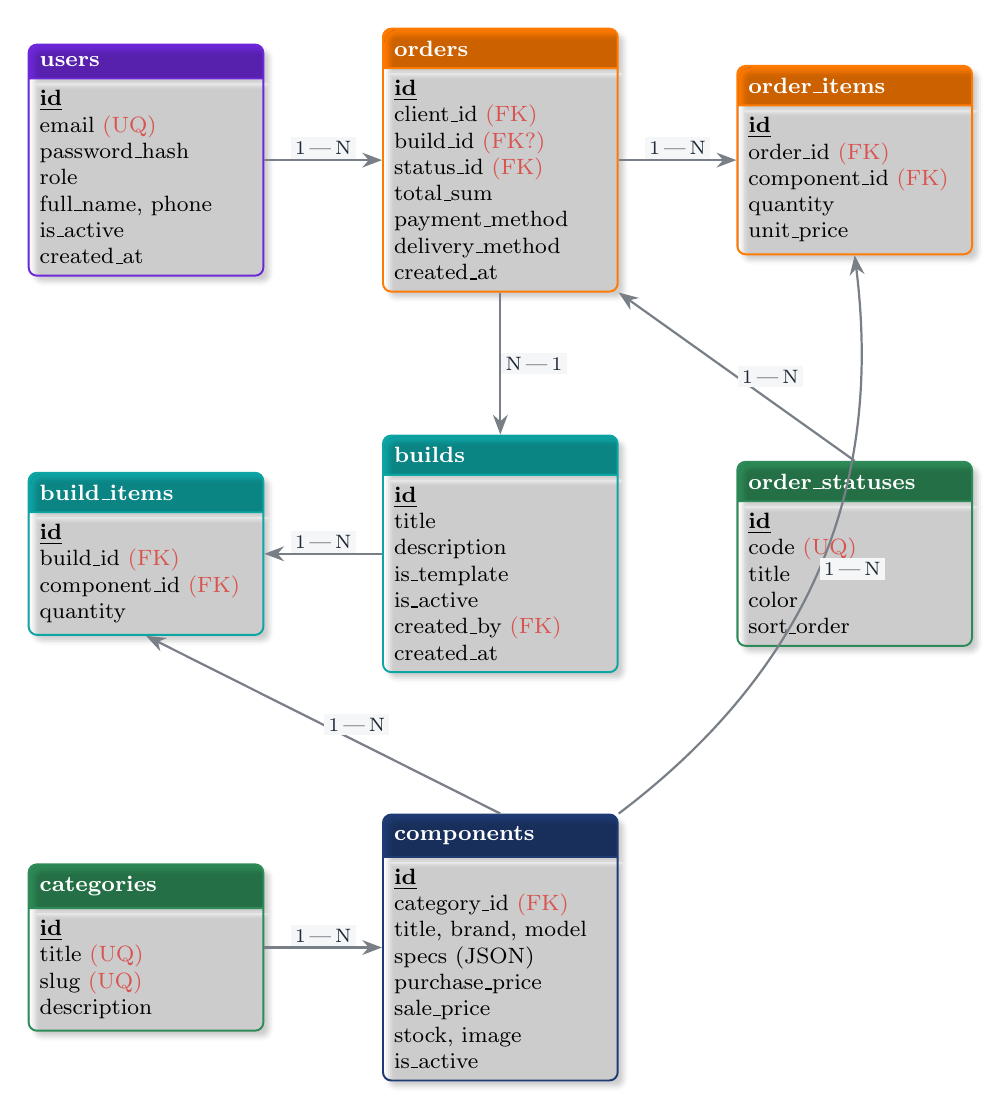
\begin{tikzpicture}[
    every node/.style={font=\footnotesize},
    entity/.style 2 args={
        draw=#1, line width=0.7pt,
        rectangle split, rectangle split parts=2,
        rectangle split draw splits=true,
        rectangle split part fill={#1, white},
        rectangle split part align={center, left},
        rounded corners=3pt,
        text width=2.6cm,
        inner sep=4pt,
        align=left,
        blur shadow={shadow blur steps=3, shadow opacity=20},
        label={[font=\footnotesize\bfseries, text=white, name=lbl-#2]center:{}},
    },
    entUser/.style   ={draw=brandPurple, line width=0.7pt, rectangle split, rectangle split parts=2, rectangle split draw splits=true, rectangle split part fill={brandPurple, white}, rectangle split part align={center, left}, rounded corners=3pt, text width=2.7cm, inner sep=4pt, align=left, blur shadow={shadow blur steps=3, shadow opacity=20}},
    entOrder/.style  ={draw=brandOrange, line width=0.7pt, rectangle split, rectangle split parts=2, rectangle split draw splits=true, rectangle split part fill={brandOrange, white}, rectangle split part align={center, left}, rounded corners=3pt, text width=2.7cm, inner sep=4pt, align=left, blur shadow={shadow blur steps=3, shadow opacity=20}},
    entBuild/.style  ={draw=brandTeal, line width=0.7pt, rectangle split, rectangle split parts=2, rectangle split draw splits=true, rectangle split part fill={brandTeal, white}, rectangle split part align={center, left}, rounded corners=3pt, text width=2.7cm, inner sep=4pt, align=left, blur shadow={shadow blur steps=3, shadow opacity=20}},
    entProduct/.style={draw=brandBlue, line width=0.7pt, rectangle split, rectangle split parts=2, rectangle split draw splits=true, rectangle split part fill={brandBlue, white}, rectangle split part align={center, left}, rounded corners=3pt, text width=2.7cm, inner sep=4pt, align=left, blur shadow={shadow blur steps=3, shadow opacity=20}},
    entRef/.style    ={draw=brandGreen, line width=0.7pt, rectangle split, rectangle split parts=2, rectangle split draw splits=true, rectangle split part fill={brandGreen, white}, rectangle split part align={center, left}, rounded corners=3pt, text width=2.7cm, inner sep=4pt, align=left, blur shadow={shadow blur steps=3, shadow opacity=20}},
    rel/.style={font=\scriptsize, text=brandDark, fill=brandLight, inner sep=1.5pt},
    link/.style={->, draw=brandDark!60, thick, >={Stealth[length=2.5mm]}},
]
% 3 строки × 3 колонки, шаг 4.5 см по X, шаг 5 см по Y
% Верхний ряд: users, orders, order_items
\node[entUser]   (users)       at (-4.5,  0) {\textcolor{white}{\bfseries users} \nodepart{second} \underline{\textbf{id}}\\ email \textcolor{brandRed}{(UQ)}\\ password\_hash\\ role\\ full\_name, phone\\ is\_active\\ created\_at};
\node[entOrder]  (orders)      at (   0,  0) {\textcolor{white}{\bfseries orders} \nodepart{second} \underline{\textbf{id}}\\ client\_id \textcolor{brandRed}{(FK)}\\ build\_id \textcolor{brandRed}{(FK?)}\\ status\_id \textcolor{brandRed}{(FK)}\\ total\_sum\\ payment\_method\\ delivery\_method\\ created\_at};
\node[entOrder]  (order_items) at ( 4.5,  0) {\textcolor{white}{\bfseries order\_items} \nodepart{second} \underline{\textbf{id}}\\ order\_id \textcolor{brandRed}{(FK)}\\ component\_id \textcolor{brandRed}{(FK)}\\ quantity\\ unit\_price};
% Средний ряд: build_items, builds, order_statuses
\node[entBuild]  (build_items) at (-4.5, -5) {\textcolor{white}{\bfseries build\_items} \nodepart{second} \underline{\textbf{id}}\\ build\_id \textcolor{brandRed}{(FK)}\\ component\_id \textcolor{brandRed}{(FK)}\\ quantity};
\node[entBuild]  (builds)      at (   0, -5) {\textcolor{white}{\bfseries builds} \nodepart{second} \underline{\textbf{id}}\\ title\\ description\\ is\_template\\ is\_active\\ created\_by \textcolor{brandRed}{(FK)}\\ created\_at};
\node[entRef]    (statuses)    at ( 4.5, -5) {\textcolor{white}{\bfseries order\_statuses} \nodepart{second} \underline{\textbf{id}}\\ code \textcolor{brandRed}{(UQ)}\\ title\\ color\\ sort\_order};
% Нижний ряд: categories, components
\node[entRef]    (categories)  at (-4.5, -10) {\textcolor{white}{\bfseries categories} \nodepart{second} \underline{\textbf{id}}\\ title \textcolor{brandRed}{(UQ)}\\ slug \textcolor{brandRed}{(UQ)}\\ description};
\node[entProduct](components)  at (   0, -10) {\textcolor{white}{\bfseries components} \nodepart{second} \underline{\textbf{id}}\\ category\_id \textcolor{brandRed}{(FK)}\\ title, brand, model\\ specs (JSON)\\ purchase\_price\\ sale\_price\\ stock, image\\ is\_active};
% Связи
\draw[link] (users.east)            -- node[above, rel] {1\,—\,N}    (orders.west);
\draw[link] (orders.east)           -- node[above, rel] {1\,—\,N}    (order_items.west);
\draw[link] (orders.south)          -- node[right, rel] {N\,—\,1}    (builds.north);
\draw[link] (statuses.north)        -- node[right, rel] {1\,—\,N}    (orders.south east);
\draw[link] (builds.west)           -- node[above, rel] {1\,—\,N}    (build_items.east);
\draw[link] (categories.east)       -- node[above, rel] {1\,—\,N}    (components.west);
\draw[link] (components.north)      -- node[right, rel] {1\,—\,N}    (build_items.south);
\draw[link] (components.north east) to[bend right=30] node[right, rel] {1\,—\,N} (order_items.south);
\end{tikzpicture}%
}
\caption{ER-диаграмма базы данных (нотация Crow's foot)}
\label{fig:er}
\end{figure}

В таблице~\ref{tab:db} приведён перечень основных таблиц физической схемы базы данных в формате PostgreSQL, в таблицах~\ref{tab:dd-users}--\ref{tab:dd-orders} --- словари данных для трёх ключевых сущностей.

\begin{table}[ht!]
\caption{Основные таблицы базы данных}
\label{tab:db}
\small
\begin{tabularx}{\textwidth}{|>{\RaggedRight\arraybackslash}p{0.20\textwidth}|>{\RaggedRight\arraybackslash}p{0.30\textwidth}|>{\RaggedRight\arraybackslash}X|}
\hline
\textbf{Таблица} & \textbf{Назначение} & \textbf{Ключевые поля} \\ \hline
users & Учётная запись пользователя & id, email, password\_hash, role, full\_name, phone, is\_active, created\_at \\ \hline
categories & Справочник категорий комплектующих & id, title, slug, description \\ \hline
components & Комплектующие (товары) & id, category\_id, title, brand, model, specs (JSON), purchase\_price, sale\_price, stock, image \\ \hline
builds & Готовая или клиентская сборка ПК & id, title, description, total\_price, created\_by, created\_at \\ \hline
build\_items & Состав сборки & id, build\_id, component\_id, quantity \\ \hline
orders & Заказ клиента & id, client\_id, build\_id, total\_sum, status, payment\_method, created\_at \\ \hline
order\_items & Позиции заказа & id, order\_id, component\_id, quantity, unit\_price \\ \hline
order\_statuses & Справочник статусов заказа & id, code, title, color \\ \hline
\end{tabularx}
\end{table}

\begin{table}[ht!]
\caption{Словарь данных таблицы \texttt{users}}
\label{tab:dd-users}
\small
\begin{tabularx}{\textwidth}{|>{\RaggedRight\arraybackslash}p{0.22\textwidth}|>{\RaggedRight\arraybackslash}p{0.20\textwidth}|>{\RaggedRight\arraybackslash}X|}
\hline
\textbf{Поле} & \textbf{Тип} & \textbf{Назначение и ограничения} \\ \hline
id & SERIAL PK & Первичный ключ \\ \hline
email & VARCHAR(254) UQ NOT NULL & Логин пользователя, индекс \\ \hline
password\_hash & VARCHAR(128) NOT NULL & Хэш пароля (PBKDF2) \\ \hline
role & VARCHAR(16) NOT NULL & client / manager / admin \\ \hline
full\_name & VARCHAR(150) & Полное имя пользователя \\ \hline
phone & VARCHAR(20) & Контактный телефон \\ \hline
is\_active & BOOLEAN DEFAULT TRUE & Активна ли учётная запись \\ \hline
created\_at & TIMESTAMP NOT NULL & Дата создания записи \\ \hline
\end{tabularx}
\end{table}

\begin{table}[ht!]
\caption{Словарь данных таблицы \texttt{components}}
\label{tab:dd-components}
\small
\begin{tabularx}{\textwidth}{|>{\RaggedRight\arraybackslash}p{0.22\textwidth}|>{\RaggedRight\arraybackslash}p{0.20\textwidth}|>{\RaggedRight\arraybackslash}X|}
\hline
\textbf{Поле} & \textbf{Тип} & \textbf{Назначение и ограничения} \\ \hline
id & SERIAL PK & Первичный ключ \\ \hline
category\_id & INT FK & Ссылка на categories.id \\ \hline
title & VARCHAR(200) NOT NULL & Наименование товара \\ \hline
brand & VARCHAR(100) & Производитель \\ \hline
model & VARCHAR(100) & Модель \\ \hline
specs & JSONB & Технические характеристики \\ \hline
purchase\_price & NUMERIC(10,2) & Закупочная цена \\ \hline
sale\_price & NUMERIC(10,2) NOT NULL & Продажная цена, не менее 0 \\ \hline
stock & INT NOT NULL DEFAULT 0 & Текущий остаток на складе \\ \hline
image & VARCHAR(255) & Путь к изображению товара \\ \hline
\end{tabularx}
\end{table}

\begin{table}[ht!]
\caption{Словарь данных таблицы \texttt{orders}}
\label{tab:dd-orders}
\small
\begin{tabularx}{\textwidth}{|>{\RaggedRight\arraybackslash}p{0.22\textwidth}|>{\RaggedRight\arraybackslash}p{0.20\textwidth}|>{\RaggedRight\arraybackslash}X|}
\hline
\textbf{Поле} & \textbf{Тип} & \textbf{Назначение и ограничения} \\ \hline
id & SERIAL PK & Первичный ключ \\ \hline
client\_id & INT FK NOT NULL & Ссылка на users.id \\ \hline
build\_id & INT FK NULL & Опциональная ссылка на сборку \\ \hline
total\_sum & NUMERIC(12,2) NOT NULL & Итоговая сумма заказа \\ \hline
status & VARCHAR(16) NOT NULL & Код статуса заказа \\ \hline
payment\_method & VARCHAR(20) NOT NULL & Способ оплаты \\ \hline
delivery\_method & VARCHAR(20) NOT NULL & Способ получения \\ \hline
delivery\_address & VARCHAR(255) & Адрес доставки \\ \hline
created\_at & TIMESTAMP NOT NULL & Дата оформления заказа \\ \hline
updated\_at & TIMESTAMP NOT NULL & Дата последнего обновления \\ \hline
\end{tabularx}
\end{table}

Между сущностями устанавливаются следующие связи:
\begin{itemize}
    \item \emph{Категория} --- \emph{Комплектующее}: один ко многим;
    \item \emph{Сборка} --- \emph{Состав сборки} --- \emph{Комплектующее}: «многие ко многим» через таблицу \texttt{build\_\allowbreak items};
    \item \emph{Пользователь (клиент)} --- \emph{Заказ}: один ко многим;
    \item \emph{Заказ} --- \emph{Позиция заказа} --- \emph{Комплектующее}: «многие ко многим» через таблицу \texttt{order\_\allowbreak items};
    \item \emph{Заказ} --- \emph{Сборка}: необязательная связь «многие к одному»;
    \item \emph{Заказ} --- \emph{Статус заказа}: «многие к одному» через справочник \texttt{order\_\allowbreak statuses}.
\end{itemize}

\textbf{Индексы и оптимизация запросов.} Для обеспечения быстрого поиска и фильтрации в каталоге товаров предусмотрены индексы по полям:
\begin{itemize}
    \item \texttt{components}\,.\,\texttt{category\_id} и \texttt{components}\,.\,\texttt{brand} --- для фильтров каталога;
    \item GIN-индекс по полю \texttt{components}\,.\,\texttt{specs} (JSONB) --- для поиска по техническим характеристикам;
    \item \texttt{orders}\,.\,\texttt{client\_id} и \texttt{orders}\,.\,\texttt{created\_at} --- для отчётности и личного кабинета;
    \item уникальный индекс по полю \texttt{users}\,.\,\texttt{email} --- для быстрой авторизации и предотвращения дублирования учётных записей.
\end{itemize}

Физическая реализация осуществляется средствами миграций Django, что обеспечивает воспроизводимость структуры на любой среде разработки и развёртывания.

\subsection{Разработка макетов страниц}

На основе сформулированных функциональных требований, пользовательских сценариев и спроектированной модели данных разработаны макеты основных страниц веб-приложения. Прототипы выполняются в инструменте Figma. Основные страницы сгруппированы по ролям пользователей и связаны между собой картой переходов (таблица~\ref{tab:sitemap}).

\begin{table}[ht!]
\caption{Карта сайта по ролям пользователей}
\label{tab:sitemap}
\small
\begin{tabularx}{\textwidth}{|>{\RaggedRight\arraybackslash}p{0.22\textwidth}|>{\RaggedRight\arraybackslash}p{0.20\textwidth}|>{\RaggedRight\arraybackslash}X|}
\hline
\textbf{Раздел} & \textbf{Доступ} & \textbf{Состав страниц} \\ \hline
Публичная часть & Все & Главная, каталог, карточка товара, конфигуратор, регистрация, авторизация \\ \hline
Личный кабинет клиента & Клиент, Админ & Дашборд, активные заказы, история, профиль, корзина \\ \hline
Рабочее место менеджера & Менеджер, Админ & Рабочий стол, каталог, сборки, заказы, импорт/экспорт, отчёты \\ \hline
Панель администратора & Админ & Пользователи, роли, справочники, аналитика, журнал \\ \hline
\end{tabularx}
\end{table}

\emph{Главная страница} (рисунок~\ref{fig:wf-home}) состоит из «шапки» с логотипом и ссылками на каталог и конфигуратор, «героя» с описанием магазина и кнопкой «Собрать ПК», блока популярных сборок, блока акций и «подвала» со ссылками на разделы.

\begin{figure}[ht!]
\centering
\begin{tikzpicture}[
    wfHeader/.style={draw=brandBlue, line width=0.6pt, rectangle, rounded corners=4pt, fill=brandBlue, text=white, align=center, font=\small\bfseries, minimum height=0.8cm},
    wfHero/.style={draw=brandOrange, line width=0.6pt, rectangle, rounded corners=6pt, fill=brandOrangeSoft, align=center, font=\small, minimum height=0.7cm},
    wfBtn/.style={draw=brandOrange, line width=0.5pt, rectangle, rounded corners=4pt, fill=brandOrange, text=white, align=center, font=\small\bfseries},
    wfCard/.style={draw=brandBlue!30, line width=0.5pt, rectangle, rounded corners=4pt, fill=white, align=center, font=\footnotesize, blur shadow={shadow blur steps=3, shadow opacity=15}},
    wfCardAccent/.style={draw=brandTeal!50, line width=0.5pt, rectangle, rounded corners=4pt, fill=brandTealSoft, align=center, font=\footnotesize, blur shadow={shadow blur steps=3, shadow opacity=15}},
    wfFooter/.style={draw=brandDark!30, line width=0.5pt, rectangle, rounded corners=4pt, fill=brandLight, align=center, font=\footnotesize, text=brandDark, minimum height=0.7cm},
    wfLabel/.style={font=\small\bfseries, text=brandBlue, anchor=west},
]
\node[wfHeader, minimum width=14cm] at (0, 4) {Header: лого \ \ Каталог \ \ Конфигуратор \ \ Поиск \ \ Войти / Регистрация};
\node[wfHero, minimum width=14cm, minimum height=2cm] at (0, 2.3) {«Соберите свой ПК под задачу»};
\node[wfBtn, minimum width=3cm] at (4.5, 2.0) {Собрать ПК};
\node[wfLabel] at (-7.0, 0.9) {Категории комплектующих};
\node[wfCard, minimum width=3.2cm, minimum height=0.9cm] at (-5.3, 0.0) {CPU};
\node[wfCard, minimum width=3.2cm, minimum height=0.9cm] at (-1.8, 0.0) {GPU};
\node[wfCard, minimum width=3.2cm, minimum height=0.9cm] at ( 1.8, 0.0) {RAM};
\node[wfCard, minimum width=3.2cm, minimum height=0.9cm] at ( 5.3, 0.0) {SSD};
\node[wfLabel] at (-7.0, -1.1) {Готовые сборки};
\node[wfCardAccent, minimum width=4.3cm, minimum height=1.6cm] at (-4.7, -2.2) {Сборка 1\\\textbf{74\,990~руб.} • [ Купить ]};
\node[wfCardAccent, minimum width=4.3cm, minimum height=1.6cm] at ( 0.0, -2.2) {Сборка 2\\\textbf{105\,000~руб.} • [ Купить ]};
\node[wfCardAccent, minimum width=4.3cm, minimum height=1.6cm] at ( 4.7, -2.2) {Сборка 3\\\textbf{152\,500~руб.} • [ Купить ]};
\node[wfFooter, minimum width=14cm] at (0, -3.5) {Footer: контакты, соцсети, © pcshop};
\end{tikzpicture}
\caption{Wireframe главной страницы}
\label{fig:wf-home}
\end{figure}

\emph{Каталог товаров} (рисунок~\ref{fig:wf-catalog}) содержит панель фильтров слева (категория, цена, бренд, характеристики, остаток) и сетку карточек с пагинацией. Каждая карточка показывает изображение, наименование, бренд, цену, остаток и кнопку «Добавить в корзину».

\begin{figure}[ht!]
\centering
\begin{tikzpicture}[
    wfHeader/.style={draw=brandBlue, line width=0.6pt, rectangle, rounded corners=4pt, fill=brandBlue, text=white, align=center, font=\small\bfseries, minimum height=0.8cm},
    wfFilters/.style={draw=brandBlue!40, line width=0.5pt, rectangle, rounded corners=4pt, fill=brandBlueSoft, align=left, font=\footnotesize, inner sep=6pt, blur shadow={shadow blur steps=3, shadow opacity=15}},
    wfCard/.style={draw=brandBlue!30, line width=0.5pt, rectangle, rounded corners=4pt, fill=white, align=center, font=\footnotesize, blur shadow={shadow blur steps=3, shadow opacity=15}},
    wfPager/.style={draw=brandDark!30, line width=0.5pt, rectangle, rounded corners=4pt, fill=brandLight, align=center, font=\footnotesize, minimum height=0.7cm},
]
\node[wfHeader, minimum width=14cm] at (0, 4) {Header / Хлебные крошки: Главная $\rightarrow$ Каталог $\rightarrow$ Процессоры};
\node[wfFilters, minimum width=3.8cm, minimum height=6cm, anchor=north west] at (-7, 3.4) {
    \textbf{\textcolor{brandBlue}{Фильтры}}\\[4pt]
    $\square$ Категория\\
    $\square$ Бренд\\[4pt]
    \textcolor{brandDark}{Цена,~руб.}\\
    {[\,\_\_\_]\,—\,[\,\_\_\_]}\\[4pt]
    $\square$ В наличии\\
    $\square$ Низкий остаток\\[6pt]
    \textcolor{brandOrange}{\textbf{[ Применить ]}}
};
\foreach \xi/\yi/\n in {-1.7/2.4/1, 1.5/2.4/2, 4.7/2.4/3, -1.7/0/4, 1.5/0/5, 4.7/0/6} {
    \node[wfCard, minimum width=2.8cm, minimum height=2.2cm] at (\xi, \yi) {Карточка\\товара \n\\\\\textbf{\textcolor{brandOrange}{цена~руб.}}\\{[ В корзину ]}};
}
\node[wfPager, minimum width=9.5cm] at (1.5, -1.6) {Пагинация: \ \ \textbf{\textcolor{brandBlue}{1}} \ 2 \ 3 \ \ldots \ N};
\end{tikzpicture}
\caption{Wireframe страницы каталога товаров}
\label{fig:wf-catalog}
\end{figure}

\emph{Конфигуратор сборки} (рисунок~\ref{fig:wf-config}) реализован как пошаговый мастер с подсветкой активного шага. На каждом шаге отображается панель выбора одной категории комплектующих, под ней --- сводка текущей сборки и итоговая сумма.

\begin{figure}[ht!]
\centering
\begin{tikzpicture}[
    wfHeader/.style={draw=brandBlue, line width=0.6pt, rectangle, rounded corners=4pt, fill=brandBlue, text=white, align=center, font=\small\bfseries, minimum height=0.8cm},
    wstep/.style={draw=brandBlue!40, line width=0.5pt, rectangle, rounded corners=4pt, fill=brandBlueSoft, text=brandBlue, align=center, font=\footnotesize, minimum height=0.6cm, minimum width=1.5cm},
    wstepActive/.style={draw=brandOrange, line width=0.7pt, rectangle, rounded corners=4pt, fill=brandOrange, text=white, align=center, font=\footnotesize\bfseries, minimum height=0.6cm, minimum width=1.5cm, blur shadow={shadow blur steps=3, shadow opacity=20}},
    wstepDone/.style={draw=brandGreen, line width=0.5pt, rectangle, rounded corners=4pt, fill=brandGreenSoft, text=brandGreen, align=center, font=\footnotesize\bfseries, minimum height=0.6cm, minimum width=1.5cm},
    panel/.style={draw=brandBlue!30, line width=0.5pt, rectangle, rounded corners=6pt, fill=white, align=left, font=\footnotesize, inner sep=8pt, blur shadow={shadow blur steps=3, shadow opacity=15}},
    summary/.style={draw=brandOrange!60, line width=0.7pt, rectangle, rounded corners=6pt, fill=brandOrangeSoft, align=left, font=\footnotesize, inner sep=8pt, blur shadow={shadow blur steps=3, shadow opacity=20}},
    navBtn/.style={draw=brandDark!30, line width=0.5pt, rectangle, rounded corners=4pt, fill=white, align=center, font=\footnotesize, minimum height=0.7cm, minimum width=3cm},
    navBtnPrimary/.style={draw=brandOrange, line width=0.5pt, rectangle, rounded corners=4pt, fill=brandOrange, text=white, align=center, font=\footnotesize\bfseries, minimum height=0.7cm, minimum width=3cm},
]
\node[wfHeader, minimum width=14cm] at (0, 3.7) {Конфигуратор сборки ПК};
\node[wstepDone]   at (-5.8, 2.6) {1. CPU};
\node[wstepActive] at (-3.9, 2.6) {2. MB};
\node[wstep]       at (-2.0, 2.6) {3. RAM};
\node[wstep]       at (-0.1, 2.6) {4. SSD};
\node[wstep]       at ( 1.8, 2.6) {5. GPU};
\node[wstep]       at ( 3.7, 2.6) {6. PSU};
\node[wstep]       at ( 5.6, 2.6) {7. Корпус};
\node[panel, minimum width=9cm, minimum height=3.2cm, anchor=north west] at (-7, 1.8) {
    \textbf{\textcolor{brandBlue}{Шаг 2. Материнская плата}}\\[4pt]
    Фильтры: форм-фактор, чипсет, тип памяти, Wi-Fi.\\[4pt]
    {[ Карточка платы 1 ] \ [ Карточка 2 ] \ [ Карточка 3 ]}\\
    {[ Карточка платы 4 ] \ [ Карточка 5 ] \ [ Карточка 6 ]}\\[4pt]
    \textcolor{brandOrange}{\textbf{[ Выбрать ]}}
};
\node[summary, minimum width=4.4cm, minimum height=3.2cm, anchor=north west] at ( 2.6, 1.8) {
    \textbf{\textcolor{brandOrange}{Текущая сборка}}\\[4pt]
    CPU: AMD 7700X \checkmark\\
    MB: \emph{выбирается}\\
    RAM: \_\_\_\\
    SSD: \_\_\_\\
    GPU: \_\_\_\\[4pt]
    \textbf{Итого: 27\,990~руб.}
};
\node[navBtn]        at (-5.0, -2.5) {[ Назад ]};
\node[navBtn]        at (-1.5, -2.5) {Сохранить сборку};
\node[navBtnPrimary] at ( 2.0, -2.5) {Далее};
\node[navBtnPrimary] at ( 5.5, -2.5) {Оформить заказ};
\end{tikzpicture}
\caption{Wireframe конфигуратора сборки ПК}
\label{fig:wf-config}
\end{figure}

\emph{Корзина и оформление заказа} (рисунок~\ref{fig:wf-cart}) объединяет список добавленных товаров и сборок с возможностью изменения количества и удаления. Оформление выполняется одной страницей с секциями «Контактные данные», «Способ оплаты», «Способ получения» и итоговым блоком с кнопкой «Оформить заказ».

\begin{figure}[ht!]
\centering
\begin{tikzpicture}[
    wfHeader/.style={draw=brandBlue, line width=0.6pt, rectangle, rounded corners=4pt, fill=brandBlue, text=white, align=center, font=\small\bfseries, minimum height=0.8cm},
    panel/.style={draw=brandBlue!30, line width=0.5pt, rectangle, rounded corners=6pt, fill=white, align=left, font=\footnotesize, inner sep=8pt, blur shadow={shadow blur steps=3, shadow opacity=15}},
    summary/.style={draw=brandOrange!60, line width=0.8pt, rectangle, rounded corners=6pt, fill=brandOrangeSoft, align=left, font=\footnotesize, inner sep=8pt, blur shadow={shadow blur steps=3, shadow opacity=20}},
    cta/.style={draw=brandOrange, line width=0.7pt, rectangle, rounded corners=4pt, fill=brandOrange, text=white, align=center, font=\footnotesize\bfseries, minimum height=0.8cm, minimum width=3.3cm},
]
\node[wfHeader, minimum width=14cm] at (0, 3.7) {Корзина и оформление заказа};
\node[panel, minimum width=8.6cm, minimum height=2.2cm, anchor=north west] at (-7, 2.7) {
    \textbf{\textcolor{brandBlue}{Товары в корзине}}\\[3pt]
    1. \, Ryzen 7 7700X \, --- \, \textbf{27\,990~руб.} \, {[\,$-$ 1 $+$\,]} \, {[\,удалить\,]}\\
    2. \, Сборка «Игровая средняя» \, --- \, \textbf{110\,000~руб.} \, {[\,удалить\,]}
};
\node[panel, minimum width=8.6cm, minimum height=3cm, anchor=north west] at (-7, 0.2) {
    \textbf{\textcolor{brandBlue}{Контактные данные и доставка}}\\[3pt]
    Email: \, \rule{4cm}{0.4pt}\\
    Телефон: \, \rule{3.6cm}{0.4pt}\\[2pt]
    \textbf{\textcolor{brandOrange}{Оплата:}} \ $\bullet$\,Картой \quad $\circ$\,СБП \quad $\circ$\,Наличные\\
    \textbf{\textcolor{brandOrange}{Получение:}} \ $\bullet$\,Самовывоз \quad $\circ$\,Курьер
};
\node[summary, minimum width=4.6cm, minimum height=5.3cm, anchor=north west] at ( 2.2, 2.7) {
    \textbf{\textcolor{brandOrange}{Итого}}\\[4pt]
    Товары: 137\,990~руб.\\
    Доставка: 0~руб.\\[6pt]
    \rule{4cm}{0.4pt}\\[4pt]
    \textbf{Сумма: \textcolor{brandBlue}{137\,990~руб.}}\\[12pt]
};
\node[cta] at (4.5, -1.6) {[ Оформить заказ ]};
\end{tikzpicture}
\caption{Wireframe корзины и оформления заказа}
\label{fig:wf-cart}
\end{figure}

\emph{Личный кабинет клиента} (рисунок~\ref{fig:wf-client}) включает виджеты «Активные заказы» и «Сохранённые сборки», подробные блоки «История заказов» (таблица с фильтрами) и «Адреса доставки».

\begin{figure}[ht!]
\centering
\begin{tikzpicture}[
    wfHeader/.style={draw=brandBlue, line width=0.6pt, rectangle, rounded corners=4pt, fill=brandBlue, text=white, align=center, font=\small\bfseries, minimum height=0.8cm},
    sidebar/.style={draw=brandBlue!40, line width=0.5pt, rectangle, rounded corners=6pt, fill=brandBlueSoft, align=left, font=\footnotesize, inner sep=8pt, blur shadow={shadow blur steps=3, shadow opacity=15}},
    widgetA/.style={draw=brandBlue!40, line width=0.5pt, rectangle, rounded corners=6pt, fill=white, align=center, font=\footnotesize, minimum height=2.2cm, blur shadow={shadow blur steps=3, shadow opacity=15}},
    widgetB/.style={draw=brandTeal!50, line width=0.5pt, rectangle, rounded corners=6pt, fill=brandTealSoft, align=center, font=\footnotesize, minimum height=2.2cm, blur shadow={shadow blur steps=3, shadow opacity=15}},
    widgetC/.style={draw=brandGreen!50, line width=0.5pt, rectangle, rounded corners=6pt, fill=brandGreenSoft, align=center, font=\footnotesize, minimum height=2.4cm, blur shadow={shadow blur steps=3, shadow opacity=15}},
    widgetD/.style={draw=brandOrange!60, line width=0.5pt, rectangle, rounded corners=6pt, fill=brandOrangeSoft, align=center, font=\footnotesize, minimum height=2.4cm, blur shadow={shadow blur steps=3, shadow opacity=15}},
]
\node[wfHeader, minimum width=14cm] at (0, 3.7) {Личный кабинет клиента};
\node[sidebar, minimum width=3.2cm, minimum height=5.4cm, anchor=north west] at (-7, 2.7) {
    \textbf{\textcolor{brandBlue}{Меню}}\\[4pt]
    \textcolor{brandOrange}{$\bullet$ Дашборд}\\
    $\bullet$ Активные заказы\\
    $\bullet$ История\\
    $\bullet$ Сохранённые сборки\\
    $\bullet$ Адреса\\
    $\bullet$ Профиль
};
\node[widgetA, minimum width=4.6cm] at (-1.2, 1.5) {Активные заказы\\[4pt]\textbf{\textcolor{brandBlue}{\Huge 2}}};
\node[widgetB, minimum width=4.6cm] at ( 3.5, 1.5) {Сохранённые сборки\\[4pt]\textbf{\textcolor{brandTeal}{\Huge 5}}};
\node[widgetC, minimum width=4.6cm] at (-1.2, -1.6) {История заказов\\(таблица с фильтрами)};
\node[widgetD, minimum width=4.6cm] at ( 3.5, -1.6) {Адреса доставки};
\end{tikzpicture}
\caption{Wireframe личного кабинета клиента}
\label{fig:wf-client}
\end{figure}

\emph{Рабочее место менеджера} (рисунок~\ref{fig:wf-manager}) включает виджеты «Новые заказы», «В работе», «Низкие остатки», а также таблицу заказов с поиском и фильтрами. Через основное меню доступны страницы каталога, сборок, импорта/экспорта и отчётов.

\begin{figure}[ht!]
\centering
\begin{tikzpicture}[
    wfHeader/.style={draw=brandOrange, line width=0.6pt, rectangle, rounded corners=4pt, fill=brandOrange, text=white, align=center, font=\small\bfseries, minimum height=0.8cm},
    sidebar/.style={draw=brandOrange!50, line width=0.5pt, rectangle, rounded corners=6pt, fill=brandOrangeSoft, align=left, font=\footnotesize, inner sep=8pt, blur shadow={shadow blur steps=3, shadow opacity=15}},
    widgetA/.style={draw=brandBlue!40, line width=0.5pt, rectangle, rounded corners=6pt, fill=brandBlueSoft, align=center, font=\footnotesize, minimum height=1.8cm, blur shadow={shadow blur steps=3, shadow opacity=15}},
    widgetW/.style={draw=brandTeal!50, line width=0.5pt, rectangle, rounded corners=6pt, fill=brandTealSoft, align=center, font=\footnotesize, minimum height=1.8cm, blur shadow={shadow blur steps=3, shadow opacity=15}},
    widgetWarn/.style={draw=brandRed, line width=0.7pt, rectangle, rounded corners=6pt, fill=brandRedSoft, align=center, font=\footnotesize, minimum height=1.8cm, blur shadow={shadow blur steps=3, shadow opacity=20}},
    tablePanel/.style={draw=brandBlue!30, line width=0.5pt, rectangle, rounded corners=6pt, fill=white, align=center, font=\footnotesize, blur shadow={shadow blur steps=3, shadow opacity=15}},
]
\node[wfHeader, minimum width=14cm] at (0, 3.7) {Рабочее место менеджера};
\node[sidebar, minimum width=3.2cm, minimum height=5.8cm, anchor=north west] at (-7, 2.7) {
    \textbf{\textcolor{brandOrange}{Меню}}\\[4pt]
    \textcolor{brandBlue}{$\bullet$ Рабочий стол}\\
    $\bullet$ Каталог\\
    $\bullet$ Сборки\\
    $\bullet$ Заказы\\
    $\bullet$ Импорт / экспорт\\
    $\bullet$ Отчёты
};
\node[widgetA,    minimum width=3.0cm] at (-1.9, 1.5) {Новые заказы\\[4pt]\textbf{\textcolor{brandBlue}{\Huge 5}}};
\node[widgetW,    minimum width=3.0cm] at ( 1.5, 1.5) {В работе\\[4pt]\textbf{\textcolor{brandTeal}{\Huge 12}}};
\node[widgetWarn, minimum width=3.0cm] at ( 4.9, 1.5) {Низкие остатки\\[4pt]\textbf{\textcolor{brandRed}{\Huge 3}}};
\node[tablePanel, minimum width=10cm, minimum height=3cm] at (1.5, -1.4) {
    \textbf{\textcolor{brandBlue}{Таблица заказов}}: поиск, фильтры, статусы\\[8pt]
    \begin{tabular}{|c|l|c|c|c|}
        \hline
        \textbf{№} & \textbf{Клиент} & \textbf{Сумма} & \textbf{Статус} & \textbf{Действия} \\ \hline
        1021 & ivanov@... & 74\,990 & \textcolor{brandBlue}{Новый}    & [...] \\ \hline
        1020 & petrov@... & 102\,500 & \textcolor{brandOrange}{В работе} & [...] \\ \hline
    \end{tabular}
};
\end{tikzpicture}
\caption{Wireframe рабочего места менеджера}
\label{fig:wf-manager}
\end{figure}

\emph{Панель администратора} (рисунок~\ref{fig:wf-admin}) включает разделы «Пользователи», «Справочники», «Аналитика» и «Журнал действий». Основной экран аналитики содержит графики выручки и прибыли, таблицу топ-товаров и фильтры по периоду.

\begin{figure}[ht!]
\centering
\begin{tikzpicture}[
    wfHeader/.style={draw=brandPurple, line width=0.6pt, rectangle, rounded corners=4pt, fill=brandPurple, text=white, align=center, font=\small\bfseries, minimum height=0.8cm},
    sidebar/.style={draw=brandPurple!50, line width=0.5pt, rectangle, rounded corners=6pt, fill=brandPurpleSoft, align=left, font=\footnotesize, inner sep=8pt, blur shadow={shadow blur steps=3, shadow opacity=15}},
    chartBlue/.style={draw=brandBlue!40, line width=0.5pt, rectangle, rounded corners=6pt, fill=brandBlueSoft, align=center, font=\footnotesize, minimum height=2.8cm, blur shadow={shadow blur steps=3, shadow opacity=15}},
    chartGreen/.style={draw=brandGreen!50, line width=0.5pt, rectangle, rounded corners=6pt, fill=brandGreenSoft, align=center, font=\footnotesize, minimum height=2.8cm, blur shadow={shadow blur steps=3, shadow opacity=15}},
    tablePanel/.style={draw=brandPurple!30, line width=0.5pt, rectangle, rounded corners=6pt, fill=white, align=center, font=\footnotesize, blur shadow={shadow blur steps=3, shadow opacity=15}},
]
\node[wfHeader, minimum width=14cm] at (0, 3.7) {Панель администратора};
\node[sidebar, minimum width=3.2cm, minimum height=5.8cm, anchor=north west] at (-7, 2.7) {
    \textbf{\textcolor{brandPurple}{Меню}}\\[4pt]
    $\bullet$ Пользователи\\
    $\bullet$ Справочники\\
    \textcolor{brandOrange}{$\bullet$ Аналитика}\\
    $\bullet$ Журнал\\
    $\bullet$ Настройки
};
\node[chartBlue, minimum width=4.7cm] (ch1) at (-1.4, 1.4) {};
\node[font=\footnotesize\bfseries, text=brandBlue, anchor=north] at (ch1.north) {\,График выручки};
\begin{scope}[shift={(ch1.center)}, xshift=-1.7cm, yshift=-0.5cm]
    \draw[brandBlue!30, thin] (0,0) -- (3.4,0);
    \draw[brandBlue!30, thin] (0,0) -- (0,1.2);
    \draw[brandBlue, line width=1pt] (0,0.2) -- (0.7,0.6) -- (1.4,0.4) -- (2.1,0.9) -- (2.8,1.1) -- (3.4,0.7);
    \foreach \x/\y in {0/0.2, 0.7/0.6, 1.4/0.4, 2.1/0.9, 2.8/1.1, 3.4/0.7}
        \filldraw[brandBlue] (\x,\y) circle (1pt);
\end{scope}
\node[chartGreen, minimum width=4.7cm] (ch2) at ( 3.6, 1.4) {};
\node[font=\footnotesize\bfseries, text=brandGreen, anchor=north] at (ch2.north) {\,График прибыли};
\begin{scope}[shift={(ch2.center)}, xshift=-1.7cm, yshift=-0.5cm]
    \draw[brandGreen!30, thin] (0,0) -- (3.4,0);
    \foreach \x/\h in {0.2/0.6, 0.8/0.9, 1.4/0.4, 2.0/1.1, 2.6/0.8, 3.2/1.0}
        \filldraw[brandGreen] (\x,0) rectangle (\x+0.35,\h);
\end{scope}
\node[tablePanel, minimum width=10cm, minimum height=2.8cm] at (1.5, -1.6) {
    \textbf{\textcolor{brandPurple}{Топ-10 товаров за период}} \quad {\small[ Фильтр: месяц / квартал / год ]}\\[6pt]
    \begin{tabular}{|l|c|c|c|}
        \hline
        \textbf{Товар} & \textbf{Продажи} & \textbf{Выручка} & \textbf{Маржа} \\ \hline
        RTX 4070 SUPER & 24 & 1\,751\,760 & \textcolor{brandGreen}{+ 335\,760} \\ \hline
        Ryzen 7 7700X  & 31 &   867\,690 & \textcolor{brandGreen}{+ 185\,690} \\ \hline
    \end{tabular}
};
\end{tikzpicture}
\caption{Wireframe панели администратора}
\label{fig:wf-admin}
\end{figure}

При разработке макетов соблюдаются принципы: адаптивный дизайн (mobile first) на основе сетки Bootstrap~5; минимизация числа действий (оформление заказа за три перехода); единый визуальный стиль (общая цветовая палитра, типографика Roboto, набор иконок Bootstrap Icons); соблюдение требований доступности WCAG~2.1 AA; обратная связь пользователю (всплывающие уведомления, индикаторы загрузки, валидация форм). Основной цвет интерфейса --- глубокий синий (\#1F3B73), цвет акцента --- оранжевый (\#FF7A00), нейтральный фон --- светло-серый (\#F4F6F8).

Полученные результаты проектирования --- ролевая модель, функциональные требования, модель данных и макеты основных страниц --- являются исходной базой для последующей программной реализации, описанной в третьей главе пояснительной записки.

% ── Глава 3 ──────────────────────────────────────────────────────────────────
\phantomsection
\section*{Глава 3. Разработка веб-приложения}
\addcontentsline{toc}{section}{Глава 3. Разработка веб-приложения}
\stepcounter{section}

В третьей главе описывается программная реализация веб-приложения. Кодовая база организована как Django-проект \texttt{pcshop}, разделённый на четыре приложения (Django apps): \texttt{accounts} (пользователи, аутентификация и аналитика), \texttt{catalog} (категории и комплектующие), \texttt{builds} (сборки ПК, состав и конфигуратор), \texttt{orders} (корзина, заказы и статусы). Реализация выполнялась на основе официальной документации Django~\cite{django_docs} и учебных материалов~\cite{hawkins2022django}.

\subsection{Реализация базовой структуры приложения и шаблонов страниц}

Базовая структура проекта построена в соответствии с принципом «приложение на смысловую область»: каждая Django-app содержит модели, миграции, представления, формы, маршруты и админ-регистрацию своей сущности. Глобальные настройки (\texttt{settings.py}), маршрутизация (\texttt{urls.py}) и WSGI-точки входа собраны в каталоге \texttt{pcshop/}. В качестве СУБД по умолчанию используется SQLite (без дополнительной настройки), переключение на PostgreSQL выполняется через переменные окружения в файле \texttt{.env} с помощью пакета \texttt{python-decouple}.

Структура каталогов проекта приведена в таблице~\ref{tab:project-layout}.

\begin{table}[ht!]
\caption{Структура каталогов проекта \texttt{pcshop}}
\label{tab:project-layout}
\small
\begin{tabularx}{\textwidth}{|>{\RaggedRight\arraybackslash}p{0.30\textwidth}|>{\RaggedRight\arraybackslash}X|}
\hline
\textbf{Каталог / файл} & \textbf{Назначение} \\ \hline
\texttt{pcshop/} & Корневой пакет проекта: \texttt{settings.py}, \texttt{urls.py}, \texttt{views.py}, \texttt{wsgi.py} \\ \hline
\texttt{accounts/} & Пользователь, авторизация, ролевые миксины, аналитика, дашборд \\ \hline
\texttt{catalog/} & Категории, комплектующие, импорт/экспорт CSV \\ \hline
\texttt{builds/} & Сборки ПК, состав, конфигуратор \\ \hline
\texttt{orders/} & Корзина, заказы, позиции, статусы, контекст-процессор корзины \\ \hline
\texttt{templates/} & HTML-шаблоны Bootstrap~5, сгруппированные по приложениям \\ \hline
\texttt{fixtures/} & Стартовые данные (статусы заказов, категории, образцы товаров) \\ \hline
\end{tabularx}
\end{table}

\textbf{Клиентская часть} реализована на CSS-фреймворке Bootstrap~5 (подключается через CDN). Разработан единый базовый шаблон \texttt{templates/base.html}, обеспечивающий:
\begin{itemize}
    \item стек технологий Google Fonts (Inter для текста, JetBrains Mono для кода);
    \item «стеклянную» липкую навигационную панель с эффектом \texttt{backdrop-filter: blur} и адаптивным меню по ролям пользователя;
    \item единую палитру (основной цвет --- индиго \texttt{\#4F46E5}, акцент --- янтарный \texttt{\#F59E0B}), скругления, мягкие тени, hover-эффекты;
    \item современную типографику и адаптивную сетку для мобильных устройств.
\end{itemize}

Главная страница \texttt{templates/home.html} содержит hero-блок с градиентным фоном и призывом к действию, сетку категорий с иконками \texttt{Bootstrap Icons}, блок популярных сборок и блок преимуществ. Все вторичные шаблоны (каталог, корзина, личный кабинет, аналитика и др.) наследуются от базового через \texttt{\{\% extends \%\}}.

Для отображения числа позиций корзины в навигационной панели реализован контекст-процессор \texttt{orders/context\_processors.py}, зарегистрированный в \texttt{TEMPLATES[...]['OPTIONS']['context\_processors']}. Процессор читает данные только из сессии браузера (без обращений к базе данных) и добавляет переменную \texttt{cart\_count} в контекст каждого шаблона. На иконке «Корзина» отображается оранжевый числовой бейдж при наличии позиций.

\subsection{Реализация аутентификации и проверки прав доступа}

Для разграничения доступа реализована собственная модель пользователя \texttt{accounts.User}, наследующаяся от \texttt{AbstractUser}. Логин по умолчанию заменён на email: установлены \texttt{USERNAME\_FIELD = 'email'} и \texttt{REQUIRED\_FIELDS = []}, поле \texttt{username} отключено. Модель содержит поле \texttt{role} (\texttt{TextChoices}: \texttt{client}, \texttt{manager}, \texttt{admin}), а также поля \texttt{full\_name} и \texttt{phone}. Реализован собственный \texttt{UserManager}, корректно создающий обычных пользователей и суперпользователей с автоматическим назначением роли \texttt{admin}.

\textbf{Формы аутентификации.} Реализованы три ключевые формы:
\begin{itemize}
    \item \texttt{RegisterForm} (наследник \texttt{UserCreationForm}) --- регистрация клиента; роль принудительно выставляется в \texttt{client}; CSS-классы Bootstrap присваиваются автоматически в \texttt{\_\_init\_\_};
    \item \texttt{EmailAuthenticationForm} (наследник \texttt{AuthenticationForm}) --- замена \texttt{username} на \texttt{EmailField};
    \item \texttt{ProfileForm} и \texttt{BootstrapPasswordChangeForm} --- редактирование профиля и смена пароля.
\end{itemize}

\textbf{Представления.} Аутентификация реализована через class-based views: \texttt{RegisterView} (на базе \texttt{CreateView} с автоматическим логином после регистрации), \texttt{EmailLoginView}, \texttt{CustomLogoutView}, \texttt{ProfileView}, \texttt{CustomPasswordChangeView}.

\textbf{Ролевая модель доступа.} Модуль \texttt{accounts/permissions.py} содержит базовый миксин \texttt{RoleRequiredMixin}, наследующийся от \texttt{LoginRequiredMixin} и \texttt{UserPassesTestMixin}. Базовый миксин проверяет роль пользователя и предоставляет доступ суперпользователям и пользователям с ролью \texttt{admin} безусловно. От него наследуются специализированные миксины \texttt{ClientRequiredMixin}, \texttt{ManagerRequiredMixin}, \texttt{AdminRequiredMixin} и \texttt{StaffRequiredMixin} (менеджер или администратор). Для функциональных view реализованы аналогичные декораторы (\texttt{@manager\_required}, \texttt{@staff\_required} и др.). Реализация полностью соответствует матрице прав доступа, спроектированной в подразделе~2.1.

\subsection{Реализация CRUD-интерфейсов}

CRUD-операции над основными сущностями реализованы в двух плоскостях: административная панель Django для технического сопровождения и публичные/менеджерские страницы на Bootstrap~5 для основной работы пользователей.

\textbf{Каталог комплектующих.} В \texttt{catalog/views.py} реализованы:
\begin{itemize}
    \item \texttt{CatalogListView} --- публичная страница каталога с фильтрацией (поиск по названию и бренду, выбор категории, диапазон цен, наличие на складе) и пагинацией по 12 товаров;
    \item \texttt{ComponentDetailView} --- карточка товара с характеристиками из JSON-поля \texttt{specs}, ценой, остатком и кнопкой «В корзину»;
    \item \texttt{ComponentManageListView} (с миксином \texttt{StaffRequiredMixin}) --- менеджерская таблица товаров с фильтрами «низкий остаток» и категориями;
    \item \texttt{ComponentCreateView}, \texttt{ComponentUpdateView}, \texttt{ComponentDeleteView} --- стандартные CBV для CRUD с формой \texttt{ComponentForm} на Bootstrap.
\end{itemize}

\textbf{Сборки ПК.} В \texttt{builds/views.py} реализованы публичный список (\texttt{BuildListView}), детальная страница со составом сборки (\texttt{BuildDetailView}) и менеджерский CRUD с inline-formset. Класс \texttt{BuildEditView} использует \texttt{BuildItemFormSet} (\texttt{inlineformset\_factory}), что позволяет редактировать состав сборки на одной странице с самой сборкой; сохранение выполняется атомарно в одной транзакции.

\textbf{Заказы.} В \texttt{orders/views.py} реализованы:
\begin{itemize}
    \item \texttt{OrderListView} --- история заказов клиента с пагинацией;
    \item \texttt{OrderDetailView} --- детальная страница заказа с проверкой прав (клиент видит только свои заказы, менеджер и админ --- любые);
    \item \texttt{OrderManageListView} --- менеджерская таблица заказов с поиском и фильтрами по статусу;
    \item функциональное представление \texttt{manage\_change\_status} --- смена статуса заказа менеджером.
\end{itemize}

Особого внимания заслуживает функция \texttt{\_create\_order}: списание остатков реализовано через выражение \texttt{F('stock')}, что гарантирует атомарность операции на уровне СУБД и полностью исключает состояние гонки (race condition) при одновременном оформлении нескольких заказов одного товара:

\begin{lstlisting}[language=Python, caption={Атомарное списание остатков через F()-выражение}]
Component.objects.filter(pk=pk).update(stock=F('stock') - need)
\end{lstlisting}

Всё создание заказа обёрнуто в \texttt{transaction.atomic()}: при любой ошибке (нехватка остатков, ошибка записи) все изменения откатываются целиком.

\textbf{Личный кабинет (дашборд).} Представление \texttt{DashboardView} динамически формирует контекст в зависимости от роли пользователя: для клиента передаются последние 5 заказов с \texttt{select\_related('status')} (без N+1-запросов к статусам); для менеджера и администратора --- последние 10 заказов всех клиентов. Шаблон \texttt{accounts/dashboard.html} отображает: для клиента --- KPI-карточку с числом заказов, ссылки на конфигуратор и каталог, таблицу истории заказов; для менеджера --- карточки быстрого доступа к каталогу, сборкам, заказам и аналитике; для администратора --- дополнительно ссылки на управление пользователями и экспорт/импорт CSV.

\textbf{Каталог --- улучшения UX.} Страница каталога дополнена счётчиком найденных позиций в заголовке, боковой панелью быстрой фильтрации по категориям с подсветкой активной и кнопкой «Сбросить» фильтры. Пагинация реализована с сохранением GET-параметров --- переход на следующую страницу не сбрасывает выбранные фильтры (все параметры передаются через цикл в URL пагинационных ссылок).

\subsection{Реализация модуля сборки ПК из комплектующих (конфигуратор)}

Модуль конфигуратора (URL \texttt{/builds/configure/}) реализован как однострничное приложение на Alpine.js поверх Django-шаблона, что позволяет получить полностью реактивный пользовательский интерфейс без отдельной сборки фронтенда. Архитектурное решение --- frontend получает все доступные комплектующие в момент загрузки страницы (через \texttt{json\_script}) и далее работает без обращений к серверу, кроме финального сохранения сборки.

\textbf{Архитектура шагов.} В \texttt{builds/views.py} определена константа \texttt{CONFIGURATOR\_STEPS} --- список восьми шагов: процессор, материнская плата, оперативная память, накопитель, видеокарта, блок питания, корпус, охлаждение. Каждый шаг имеет поля \texttt{key}, \texttt{slug} категории, \texttt{title}, имя иконки \texttt{Bootstrap Icons} и флаг \texttt{required}. В контекст шаблона передаётся уже сгруппированный по шагам JSON со списком всех активных комплектующих с положительным остатком.

\textbf{Серверная часть} конфигуратора состоит из двух представлений:
\begin{itemize}
    \item \texttt{ConfiguratorView} (\texttt{TemplateView}) --- отдаёт страницу с шагами и JSON-данными комплектующих, отсортированных по цене;
    \item функциональное представление \texttt{configurator\_save} (\texttt{POST}, \texttt{@login\_required}) --- принимает JSON со словарём \texttt{selection} (ключ шага $\rightarrow$ id комплектующего), валидирует, создаёт \texttt{Build} и \texttt{BuildItem}'ы атомарно (\texttt{transaction.atomic}) и опционально добавляет сборку в корзину пользователя.
\end{itemize}

\textbf{Клиентская часть} реализована на Alpine.js (подключён через CDN, ${\sim}$15~КБ) с описанной далее логикой.

\emph{Реактивные компоненты:}
\begin{itemize}
    \item \texttt{steps} --- массив шагов с комплектующими, инициализируется из \texttt{json\_script};
    \item \texttt{currentStep} --- индекс текущего шага мастера;
    \item \texttt{selection} --- словарь выбранных комплектующих (синхронизируется с \texttt{localStorage});
    \item вычисляемые методы \texttt{filteredComponents()}, \texttt{isCompatible()}, \texttt{estimatedPower()}, \texttt{totalPrice()}, \texttt{canCheckout()}.
\end{itemize}

\emph{Правила совместимости} реализованы в методе \texttt{isCompatible(component)} и проверяются динамически при отрисовке каждой карточки:
\begin{enumerate}
    \item \textbf{Процессор $\leftrightarrow$ материнская плата}: сокеты должны совпадать (\texttt{cpu.specs.sockets == mb.specs.socket}).
    \item \textbf{Материнская плата $\leftrightarrow$ память}: тип памяти должен совпадать (\texttt{mb.specs.memory == ram.specs.type}; например, DDR5).
    \item \textbf{Блок питания}: расчётное энергопотребление (сумма TDP процессора, TDP видеокарты и константы 80 Вт на остальные узлы) не должно превышать мощность БП. При превышении карточка БП помечается как несовместимая, при разности менее 100 Вт выводится предупреждение «БП на пределе».
    \item \textbf{Кулер $\leftrightarrow$ процессор}: расчётный TDP кулера должен покрывать TDP процессора.
\end{enumerate}

Несовместимые позиции автоматически помечаются красным бейджем «несовместимо», приглушаются (\texttt{opacity: 0.5}) и блокируются от клика. На самой дешёвой совместимой позиции каждого шага автоматически отображается бейдж «рекомендуем».

\emph{Визуальные элементы интерфейса:}
\begin{itemize}
    \item \textbf{Пошаговый стайплер} с горизонтальной прокруткой и цветовой индикацией состояния (пустой, активный, выполненный);
    \item \textbf{Градиентный прогресс-бар} (индиго $\rightarrow$ фиолетовый $\rightarrow$ розовый), показывающий долю выполненных шагов;
    \item \textbf{Реактивная сводка справа} (\texttt{position: sticky}) с иконками шагов, выбранными комплектующими и ценами;
    \item \textbf{Индикатор мощности БП} с цветной полосой (зелёный $\rightarrow$ жёлтый $\rightarrow$ красный) и текстовой подсказкой о требуемой мощности;
    \item \textbf{Алерты совместимости} в верхней части страницы при конфликтах между выбранными элементами;
    \item \textbf{Сохранение в \texttt{localStorage}} --- при возврате на страницу пользователь видит свой предыдущий выбор.
\end{itemize}

\emph{Завершение сборки.} После выбора всех обязательных шагов разблокируются кнопки «В корзину» (с указанной суммой) и «Сохранить сборку». При нажатии выполняется \texttt{fetch}-запрос на \texttt{/builds/configure/save/} с CSRF-токеном из cookie; сервер создаёт сборку и возвращает URL для редиректа (страница сборки или корзина).

\subsection{Реализация агрегирования данных по остаткам, продажам и прибыли}

Аналитический модуль реализован в виде представления \texttt{AnalyticsView} (\texttt{accounts/views.py}) с использованием миксина \texttt{StaffRequiredMixin} (доступ только менеджерам и администраторам). Все расчёты выполняются на стороне СУБД через агрегирующие методы Django ORM, что обеспечивает приемлемую производительность даже при больших объёмах заказов.

\textbf{Период выборки} задаётся параметром \texttt{?days=N} (по умолчанию 30 дней; поддерживаются значения 7, 30, 90 и 365). Все выборки фильтруются по \texttt{created\_at}, отменённые заказы (статус \texttt{cancelled}) исключаются.

\textbf{Ключевые показатели} рассчитываются за один запрос с использованием выражений \texttt{Sum} и \texttt{F}:
\begin{itemize}
    \item \textbf{Выручка}: \texttt{Sum(F('unit\_price') * F('quantity'))};
    \item \textbf{Себестоимость}: \texttt{Sum(F('component\_\allowbreak purchase\_price') * F('quantity'))};
    \item \textbf{Прибыль}: разность выручки и себестоимости;
    \item \textbf{Количество заказов} и \textbf{средний чек}: \texttt{Count('order', distinct=True)} и отношение выручки к количеству заказов.
\end{itemize}

\textbf{Топ-10 товаров} рассчитывается группировкой позиций заказов по \texttt{component\_\allowbreak title} и \texttt{component\_\allowbreak brand} с агрегацией \texttt{Sum('quantity')} и сортировкой по убыванию. Дополнительно выгружаются позиции с критически низкими остатками и подсчитывается количество товаров «нет в наличии».

\textbf{Визуализация} построена на цветных KPI-карточках (с градиентным фоном для основных показателей), таблице топ-товаров и боковом списке низких остатков с цветными бейджами (жёлтый --- мало, красный --- нет в наличии).

\subsection{Реализация загрузки и выгрузки файлов}

Модуль импорта-экспорта реализован для каталога комплектующих и отчётности по заказам.

\textbf{Экспорт каталога} (\texttt{ComponentExportView}) --- генерирует CSV-файл с разделителем «;», кодировкой UTF-8 и предваряющим BOM (для корректного открытия в Microsoft Excel). Заголовок: \texttt{id, category, title, brand, model, specs, purchase\_price, sale\_price, stock, is\_active}. Содержимое поля \texttt{specs} (JSON) сериализуется в текстовый JSON через \texttt{json.dumps(ensure\_ascii=False)}.

\textbf{Импорт каталога} (\texttt{ComponentImportView}) --- загрузка CSV-файла через стандартный \texttt{FileField}. Алгоритм импорта:
\begin{enumerate}
    \item декодирование содержимого как \texttt{utf-8-sig} (корректная обработка BOM из Excel);
    \item чтение через \texttt{csv.DictReader} c разделителем «;»;
    \item для каждой строки --- валидация обязательных полей (категория, название);
    \item поиск или автоматическое создание категории по \texttt{slug};
    \item парсинг JSON-поля \texttt{specs};
    \item операция \texttt{Component.objects.update\_or\_create(title=...)}, что обеспечивает идемпотентность повторных загрузок.
\end{enumerate}

По завершении импорта пользователю выводится сообщение со статистикой (создано, обновлено, пропущено) и до 10 ошибок валидации в виде flash-сообщений.

\textbf{Экспорт заказов} (\texttt{OrderExportView}) --- CSV-выгрузка заказов за период с заголовком \texttt{order\_id, date, client\_email, status, total\_sum, payment\_method, delivery\_method}. Период фильтруется параметрами \texttt{?from=YYYY-MM-DD\&to=YYYY-MM-DD}.

\subsection*{Выводы по главе 3}
\addcontentsline{toc}{subsection}{Выводы по главе 3}

В главе описана программная реализация всех шести задач раздела~3 пояснительной записки. Реализованы базовая структура приложения и шаблоны страниц на Bootstrap~5 с современным дизайн-кодом, аутентификация по email и ролевая модель доступа, полноценные CRUD-интерфейсы для всех основных сущностей системы, интерактивный конфигуратор сборки ПК с проверкой совместимости в реальном времени и расчётом потребляемой мощности, аналитический модуль с расчётом выручки, прибыли, среднего чека и топ-товаров, а также модуль импорта и экспорта файлов в формате CSV. Полученная реализация полностью покрывает функциональные требования, сформулированные в подразделе~1.4.

% ── Глава 4 ──────────────────────────────────────────────────────────────────
\phantomsection
\section*{Глава 4. Оформление итогов работы}
\addcontentsline{toc}{section}{Глава 4. Оформление итогов работы}
\stepcounter{section}

В четвёртой главе описывается организация кодовой базы в системе контроля версий, тестирование и развёртывание приложения.

\subsection{Организация Git-репозитория}

Исходный код проекта размещён в публичном репозитории на платформе GitHub:

\begin{center}
\textbf{\url{https://github.com/Haskeri/kpweb}}
\end{center}

Развёрнутое веб-приложение доступно по адресу:

\begin{center}
\textbf{\url{https://exam.anufriev.pvpcult.ru/}}
\end{center}

Кодовая база проекта организована в репозитории Git. Корень репозитория содержит каталог \texttt{pcshop/} с Django-проектом, файл \texttt{requirements.txt} со списком зависимостей и файл \texttt{.gitignore}.

Репозиторий содержит полную историю разработки, сформированную в соответствии с этапами курсовой работы. История коммитов отражает последовательное выполнение разделов (таблица~\ref{tab:commits}).

\begin{table}[ht!]
\caption{История коммитов репозитория}
\label{tab:commits}
\small
\begin{tabularx}{\textwidth}{|p{0.22\textwidth}|p{0.18\textwidth}|>{\RaggedRight\arraybackslash}X|}
\hline
\textbf{Коммит} & \textbf{Дата} & \textbf{Содержание} \\ \hline
Раздел 1 & 25.04.2026 & Анализ предметной области, постановка задачи, структура LaTeX-проекта \\ \hline
Раздел 2 & 16.05.2026 & Проектирование архитектуры, схема БД, диаграммы компонентов \\ \hline
Раздел 3 & 06.06.2026 & Разработка веб-приложения, исходный код проекта pcshop (Django 4.2) \\ \hline
Раздел 4 & 13.06.2026 & Итоговый отчёт, развёртывание, оформление пояснительной записки \\ \hline
\end{tabularx}
\end{table}

Файл \texttt{.gitignore} исключает из репозитория:
\begin{itemize}
    \item виртуальное окружение \texttt{.venv/} и кэш Python \texttt{\_\_pycache\_\_/};
    \item базу данных \texttt{db.sqlite3} (содержит пользовательские данные);
    \item файл конфигурации \texttt{configs/.env} с реальными секретами;
    \item медиафайлы (загружаемые изображения комплектующих).
\end{itemize}

В репозитории хранится только файл \texttt{configs/.env.example} --- шаблон переменных окружения без реальных значений. Это обеспечивает безопасность: секреты и чувствительные настройки не попадают в историю коммитов.

Структура файла \texttt{requirements.txt} приведена в таблице~\ref{tab:requirements}.

\begin{table}[ht!]
\caption{Зависимости проекта (\texttt{requirements.txt})}
\label{tab:requirements}
\small
\begin{tabularx}{\textwidth}{|>{\RaggedRight\arraybackslash}p{0.35\textwidth}|>{\RaggedRight\arraybackslash}X|}
\hline
\textbf{Пакет} & \textbf{Назначение} \\ \hline
\texttt{Django==4.2.16} & Веб-фреймворк (LTS-версия до апреля 2026~г.) \\ \hline
\texttt{Pillow==10.3.0} & Обработка изображений (загрузка фото комплектующих) \\ \hline
\texttt{python-decouple==3.8} & Чтение конфигурации из файла \texttt{.env} \\ \hline
\texttt{psycopg2-binary==2.9.9} & Драйвер PostgreSQL (для продакшен-развёртывания) \\ \hline
\end{tabularx}
\end{table}

Установка зависимостей выполняется командой \texttt{pip install -r requirements.txt} в активированном виртуальном окружении Python 3.10+. Для инициализации базы данных и загрузки начальных данных предусмотрены команды:

\begin{lstlisting}[language=bash, caption={Команды инициализации проекта}]
python manage.py migrate
python manage.py loaddata fixtures/order_statuses.json
python manage.py loaddata fixtures/categories.json
python manage.py loaddata fixtures/components.json
python manage.py createsuperuser
\end{lstlisting}

\subsection{Тестирование и развёртывание приложения}

\textbf{Проверка системы.} Встроенная команда Django \texttt{python manage.py check} выполняет статическую проверку конфигурации, URL-маршрутов, моделей и установленных приложений. Команда \texttt{python manage.py check --deploy} дополнительно проверяет настройки безопасности (HTTPS, CSRF, SECRET\_KEY). Оба вида проверки не выявляют ошибок.

\textbf{Ручное тестирование.} Проведено функциональное тестирование всех ключевых сценариев:
\begin{itemize}
    \item регистрация нового клиента и вход по email;
    \item добавление комплектующих в корзину со страницы каталога и со страницы товара;
    \item создание сборки в конфигураторе с проверкой совместимости;
    \item оформление заказа с уменьшением остатков на складе;
    \item смена статуса заказа менеджером;
    \item экспорт и импорт каталога в формате CSV.
\end{itemize}

Все сценарии выполняются без ошибок на Python 3.9 при использовании SQLite в качестве СУБД.

\textbf{Развёртывание.} Для локального запуска используется встроенный сервер разработки:

\begin{lstlisting}[language=bash, caption={Запуск сервера разработки}]
cd pcshop
source .venv/bin/activate
python manage.py runserver
\end{lstlisting}

Приложение становится доступным по адресу \texttt{http://localhost:8000/}. Интерактивная административная панель доступна по адресу \texttt{http://localhost:8000/admin/}.

\textbf{Продакшен-развёртывание.} Помимо локального запуска, проект развёрнут на хостинге и доступен по адресу:

\begin{center}
\url{https://exam.anufriev.pvpcult.ru/}
\end{center}

На сервере используется стек: \textbf{Nginx} (обратный прокси) → \textbf{Gunicorn} (WSGI-сервер) → \textbf{Django}. Для корректной работы CSRF-защиты за HTTPS-прокси в настройках указан доверенный источник:

\begin{lstlisting}[language=bash, caption={Ключевые параметры .env на сервере}]
DEBUG=False
ALLOWED_HOSTS=exam.anufriev.pvpcult.ru
CSRF_TRUSTED_ORIGINS=https://exam.anufriev.pvpcult.ru
SECRET_KEY=<длинный случайный ключ>
\end{lstlisting}

Переход на продакшен-окружение предполагает замену SQLite на PostgreSQL через переменные окружения в \texttt{.env}:

\begin{lstlisting}[language=bash, caption={Пример файла .env для PostgreSQL}]
SECRET_KEY=your-long-random-key
DEBUG=False
ALLOWED_HOSTS=yourdomain.com
DB_ENGINE=django.db.backends.postgresql
DB_NAME=pcshop
DB_USER=pcshop_user
DB_PASSWORD=secure_password
DB_HOST=localhost
DB_PORT=5432
\end{lstlisting}

Такой подход обеспечивает принцип «12-factor app»: конфигурация полностью отделена от кода и не попадает в репозиторий.

\subsection*{Выводы по главе 4}
\addcontentsline{toc}{subsection}{Выводы по главе 4}

В четвёртой главе описана организация кодовой базы в системе Git с корректным \texttt{.gitignore}, разделением конфигурации через \texttt{.env} и фикстурами для первоначального заполнения базы данных. Исходный код размещён в публичном репозитории по адресу \url{https://github.com/Haskeri/kpweb}. Проведено ручное функциональное тестирование всех ключевых пользовательских сценариев. Приложение развёрнуто на хостинге и доступно по адресу \url{https://exam.anufriev.pvpcult.ru/}. Описаны команды запуска в режиме разработки и инструкция по переходу на продакшен-СУБД PostgreSQL без изменения кода приложения.

% ── Заключение ───────────────────────────────────────────────────────────────
\phantomsection
\section*{Заключение}
\addcontentsline{toc}{section}{Заключение}

В ходе выполнения курсовой работы было спроектировано и реализовано веб-приложение для учёта комплектующих, сборки и продажи персональных компьютеров. Поставленная цель достигнута полностью: создан готовый к внедрению программный продукт, покрывающий бизнес-процессы малой компании по продаже комплектующих и сборке ПК под заказ.

\textbf{В первой главе} проведён анализ предметной области, выполнен сравнительный обзор существующих программных продуктов (DNS, «Регард», «НИКС», «Ситилинк») и универсальных CRM/ERP-систем. Установлено, что распространённые системы ориентированы преимущественно на витрину товаров и не покрывают в комплексе задачи внутреннего учёта комплектующих, конфигурирования сборок и аналитики для малого бизнеса. Анализ программных инструментов разработки позволил обоснованно выбрать технологический стек на основе Python, Django, Bootstrap и PostgreSQL.

\textbf{Во второй главе} выполнено проектирование разрабатываемого веб-приложения: проведён анализ целевой аудитории и трёх пользовательских ролей (администратор, менеджер, клиент), построена матрица прав доступа CRUD, описаны варианты использования и оформлены 16 пользовательских историй, спроектирована модель данных на восемь сущностей с описанием связей и ограничений целостности, разработаны wireframe-макеты основных страниц приложения.

\textbf{В третьей главе} выполнена программная реализация. Разработана модульная структура Django-проекта \texttt{pcshop} из четырёх приложений, реализованы все шесть задач раздела~3:
\begin{enumerate}
    \item базовая структура приложения и шаблоны страниц на Bootstrap~5 с современным дизайн-кодом (Inter, градиентные элементы, sticky-навбар, palette \texttt{\#4F46E5}/\texttt{\#F59E0B});
    \item аутентификация по email и ролевая модель доступа с миксинами и декораторами;
    \item полноценные CRUD-интерфейсы для каталога, сборок, заказов и пользователей с пагинацией, фильтрами, поиском и inline-formset для сборок;
    \item инновационный интерактивный конфигуратор сборки ПК на Alpine.js с пошаговым мастером из восьми шагов, проверкой совместимости комплектующих (4 правила: сокеты CPU--MB, тип памяти MB--RAM, мощность БП, TDP кулера), расчётом потребляемой мощности и сохранением состояния в \texttt{localStorage};
    \item аналитический модуль с агрегированием данных через выражения \texttt{Sum} и \texttt{F}: выручка, прибыль, средний чек, топ-10 товаров и контроль остатков с цветовой индикацией;
    \item модуль импорта и экспорта файлов в формате CSV для каталога и отчётности по заказам с поддержкой BOM для корректной работы с Microsoft Excel.
\end{enumerate}

\textbf{Практическая значимость} работы заключается в создании готового к внедрению программного продукта, который может быть использован действующими магазинами комплектующих и небольшими сборщиками ПК для автоматизации ключевых бизнес-процессов и снижения операционных издержек. Архитектура приложения позволяет масштабироваться по мере роста бизнеса (поддерживается переключение на PostgreSQL без изменения кода через переменные окружения).

\textbf{Особенностью реализации} является конфигуратор сборки ПК, который в отличие от рассмотренных в первой главе аналогов (DNS, НИКС, «Регард») сочетает в себе:
\begin{itemize}
    \item реактивную проверку совместимости в момент выбора каждого компонента (без перезагрузки страницы);
    \item автоматическую рекомендацию оптимальной по цене конфигурации;
    \item расчёт энергопотребления с цветовой индикацией запаса по мощности;
    \item возможность одновременно положить готовую сборку в корзину как единый товарный позицию;
    \item сохранение прогресса в \texttt{localStorage} браузера для возврата к сборке в любой момент.
\end{itemize}

\textbf{Перспективы развития.} Дальнейшее развитие проекта предполагает:
\begin{itemize}
    \item расширение правил совместимости комплектующих (поддержка стандартов PCI Express, охлаждения корпуса, форм-факторов материнских плат);
    \item интеграцию платёжных систем (СБП, банковский эквайринг) и системы email-уведомлений на этапах оформления и смены статуса заказа;
    \item подключение картографических сервисов для расчёта стоимости и сроков доставки;
    \item внедрение системы предиктивной аналитики для прогнозирования остатков и спроса;
    \item развёртывание приложения в облачной инфраструктуре с использованием Docker и Nginx.
\end{itemize}

При разработке пояснительной записки к курсовой работе строго соблюдались требования~\cite{gost_report}, определяющие структуру и правила оформления научно-исследовательских работ.

% ── Список литературы ────────────────────────────────────────────────────────
\bibliographystyle{ugost2003}
\bibliography{refs}

% ── Приложение А ─────────────────────────────────────────────────────────────
\startappendix

\phantomsection
\section*{Приложение А. Диаграмма вариантов использования}
\addcontentsline{toc}{section}{Приложение А. Диаграмма вариантов использования}
\stepcounter{section}

\begin{figure}[ht!]
\centering
\resizebox{0.97\textwidth}{!}{%
\begin{tikzpicture}[
    actor/.style={draw=brandBlue, thick, circle, minimum size=0.9cm, fill=white, font=\small\bfseries},
    ucGuest/.style={draw=brandTeal, line width=0.7pt, ellipse, minimum width=3.8cm, minimum height=1.0cm, align=center, fill=brandTealSoft, inner sep=2pt, font=\small},
    ucClient/.style={draw=brandBlue, line width=0.7pt, ellipse, minimum width=3.8cm, minimum height=1.0cm, align=center, fill=brandBlueSoft, inner sep=2pt, font=\small},
    ucManager/.style={draw=brandOrange, line width=0.7pt, ellipse, minimum width=3.8cm, minimum height=1.0cm, align=center, fill=brandOrangeSoft, inner sep=2pt, font=\small},
    ucAdmin/.style={draw=brandPurple, line width=0.7pt, ellipse, minimum width=3.8cm, minimum height=1.0cm, align=center, fill=brandPurpleSoft, inner sep=2pt, font=\small},
    system/.style={draw=brandBlue, line width=1pt, rectangle, rounded corners=8pt, dashed, inner sep=12pt, fill=brandLight},
    >={Stealth[length=3mm]},
    line/.style={draw=brandDark!60, thick},
    rel/.style={dashed, draw=brandRed, line width=0.7pt, ->},
]
\node[ucGuest]   (browse)    at (0,  4.5) {Просмотр каталога};
\node[ucGuest]   (regauth)   at (0,  3.0) {Регистрация и авторизация};
\node[ucClient]  (configure) at (0,  1.5) {Сборка в конфигураторе};
\node[ucClient]  (cart)      at (0,  0.0) {Корзина};
\node[ucClient]  (placeord)  at (0, -1.5) {Оформление заказа};
\node[ucClient]  (history)   at (0, -3.0) {История заказов и профиль};
\node[ucManager] (mgcat)     at (5.8,  4.5) {CRUD каталога};
\node[ucManager] (mgbuilds)  at (5.8,  3.0) {CRUD сборок};
\node[ucManager] (mgorders)  at (5.8,  1.5) {Обработка заказов};
\node[ucManager] (mgio)      at (5.8,  0.0) {Импорт / экспорт CSV};
\node[ucManager] (mgstock)   at (5.8, -1.5) {Корректировка остатков};
\node[ucAdmin]   (adusers)   at (5.8, -3.0) {Управление пользователями};
\node[ucAdmin]   (adstats)   at (5.8, -4.5) {Аналитика};
\begin{scope}[on background layer]
\node[system, fit=(browse)(history)(mgcat)(adstats)] {};
\end{scope}
\node[actor, draw=brandTeal,   text=brandTeal,
    label={[font=\small, text=brandTeal]below:Гость}]      (guest)   at (-6.5,  3.7) {};
\node[actor, draw=brandBlue,   text=brandBlue,
    label={[font=\small, text=brandBlue]below:Клиент}]     (client)  at (-6.5, -0.5) {};
\node[actor, draw=brandOrange, text=brandOrange,
    label={[font=\small, text=brandOrange]below:Менеджер}] (manager) at (11.5,  1.5) {};
\node[actor, draw=brandPurple, text=brandPurple,
    label={[font=\small, text=brandPurple]below:Админ}]    (admin)   at (11.5, -3.0) {};
\draw[line, color=brandTeal]   (guest)   -- (browse);
\draw[line, color=brandTeal]   (guest)   -- (regauth);
\draw[rel] (client) -- node[above, sloped, font=\scriptsize, text=brandRed] {наследует} (guest);
\draw[line, color=brandBlue]   (client)  -- (configure);
\draw[line, color=brandBlue]   (client)  -- (cart);
\draw[line, color=brandBlue]   (client)  -- (placeord);
\draw[line, color=brandBlue]   (client)  -- (history);
\draw[line, color=brandOrange] (manager) -- (mgcat);
\draw[line, color=brandOrange] (manager) -- (mgbuilds);
\draw[line, color=brandOrange] (manager) -- (mgorders);
\draw[line, color=brandOrange] (manager) -- (mgio);
\draw[line, color=brandOrange] (manager) -- (mgstock);
\draw[rel] (admin) -- node[above, sloped, font=\scriptsize, text=brandRed] {наследует} (manager);
\draw[line, color=brandPurple] (admin)   -- (adusers);
\draw[line, color=brandPurple] (admin)   -- (adstats);
\draw[rel] (placeord) -- node[above, sloped, font=\scriptsize, text=brandRed]
    {\textless\textless include\textgreater\textgreater} (regauth);
\end{tikzpicture}%
}
\caption{Диаграмма вариантов использования системы pcshop (UML Use Case)}
\end{figure}

\end{document}
